% Compile: latexmk -pdf main.tex

\documentclass[11pt,a4paper]{article}

\usepackage[margin=2.2cm]{geometry}
\usepackage{amsmath,amssymb}
\usepackage{graphicx}
\usepackage{booktabs}
\usepackage{longtable}
\usepackage{hyperref}
\usepackage{xcolor}
\usepackage{siunitx}
\usepackage{authblk}
\usepackage{caption}
\usepackage{subcaption}
\usepackage{enumitem}
% \usepackage[numbers,sort&compress]{natbib}

\graphicspath{{figures/}}
\hypersetup{colorlinks=true,linkcolor=blue!60!black,citecolor=blue!60!black,urlcolor=blue!60!black}

\title{\textbf{Not the model you'd expect:\\
twenty-four audio networks compared to human MEG and fMRI during natural listening}}

\author[1]{Michele Esposito}
\author[2]{Bruno L. Giordano}
\affil[1]{CNRS --- \textit{affiliation to be completed}}
\affil[2]{Aix-Marseille Université, CNRS, LIS --- \textit{affiliation to be completed}}
\date{}

\begin{document}
\maketitle

\begin{abstract}
Pre-trained audio deep networks are widely used as models of human auditory cortex, yet it remains unclear which architectures best capture population neural geometry during ecologically valid listening. We compared twenty-four representational models---spanning supervised CNNs, audio transformers, speech and general-audio self-supervised learning (SSL), multimodal contrastive encoders, and acoustic baselines---against magnetoencephalography (MEG) from $N=21$ participants listening to 600 natural sounds, and against auditory functional MRI (fMRI) betas obtained through a collaboration with Maastricht University ($N$ up to 10; Glasser parcels). Alignment was quantified with leave-one-participant-out representational similarity analysis (RSA), Monte-Carlo standardized effect sizes ($R^2_{\mathrm{MC}}$), and layer-resolved variance partitioning. On MEG, a task-optimized causal multiscale recurrent network achieved the strongest sensor-level match ($R^2_{\mathrm{MC}}=30.4$), followed by compact CNNs and a high-resolution modulation-transfer-function model ($23.9$), while several frontier SSL transformers ranked below legacy AudioSet classifiers. Rankings were stable across multiple MEG time windows. Layer-wise analyses ($n=784$ layers) showed that \emph{which network} is used explains most between-model variance in alignment (training objective: 75\%), whereas \emph{which layer type} contributes modestly within networks (6\%). On fMRI, the same model zoo showed strong $R^2_{\mathrm{MC}}$ in early auditory cortex (Heschl's gyrus / belts) that collapsed toward null in STS, insula, and frontal parcels---a cortical hierarchy that MEG sensor averages alone cannot resolve. These findings challenge the assumption that the newest or largest audio models are the most brain-like, and provide a multimodal framework for linking architectural choices to human representational geometry.
\end{abstract}

\section*{Keywords}
representational similarity analysis; magnetoencephalography; functional MRI; deep neural networks; auditory cortex; natural sounds; benchmarking

\section{Introduction}

How does the human brain transform acoustic waveforms into structured representations of natural sounds? Deep neural networks (DNNs) trained on large-scale audio corpora offer a compelling computational lens: if a model's internal geometry mirrors neural population responses, it may approximate the transformations performed by auditory cortex. Yet the field lacks a common yardstick. Studies differ in stimuli, preprocessing, brain modality, and---critically---in which model families are compared. Meanwhile, the model zoo has exploded: AudioSet CNNs, audio transformers, speech SSL, general-audio SSL, and multimodal contrastive encoders all claim state-of-the-art performance on benchmark leaderboards.

Whether leaderboard rank predicts brain alignment is an open question. Recent work suggests that models scoring highly on general audio evaluations are not always the most brain-like, motivating a systematic comparison on a shared neural reference. Here we address this gap using the Aud2Sem MEG dataset: participants passively listened to hundreds of natural sounds with rich semantic structure, enabling representational similarity analysis (RSA) that compares model and brain representational dissimilarity matrices (RDMs) on identical stimuli.

We benchmarked twenty-four models at MEG sensor level and at layer resolution, tracked alignment across multiple MEG time windows, and applied variance-partition regression to ask which architectural factors---training objective, architecture family, layer class, depth---covary with brain alignment and its temporal dynamics. In parallel, we extended the same model zoo to region-of-interest (ROI) fMRI using condition-averaged betas shared through a collaboration with Maastricht University, asking whether MEG-favoured models remain brain-like across the auditory cortical hierarchy. Our central question is practical and theoretical: \emph{when listening to natural sounds, which audio AI models actually look like the brain---and why?}

\section{Results}

\subsection{Supervised and hand-crafted models outperform frontier SSL transformers}

We evaluated brain alignment for twenty-four representational models (22 DNNs plus two acoustic baselines and an externally validated causal recurrent benchmark). For each model, layer-wise RDM predictors were combined and regressed against whitened crossnobis sensor RDMs at each MEG time point using leave-one-participant-out (LOPO) cross-validation. Integration-window scores (200--350\,ms post-onset) were expressed as Monte-Carlo standardized $R^2_{\mathrm{MC}}$ (20 null splits $\times$ 500 surrogate RDMs; baseline-corrected over pre-stimulus time).

Table~\ref{tab:leaderboard} ranks all models. The top performer was a supervised causal multiscale recurrent network (MSCRNN) trained on cochleagrams ($R^2_{\mathrm{MC}}=30.4$), ahead of a compact CNN (PANNs\_Cnn6: 24.4) and a high-resolution modulation-transfer-function (MTF) model (23.9). Several widely used frontier models---including BEATs (13.9) and EnCodecMAE (16.6)---fell below legacy AudioSet CNNs from 2017--2019. A lightweight spectrotemporal mel proxy ranked last (5.3). All models showed significant positive alignment in the integration window (sign-flip permutation test, $n_{\mathrm{perm}}=10{,}000$, family-wise error rate $\alpha=0.05$).

\begin{table}[ht]
\centering
\caption{Brain alignment leaderboard (mean $R^2_{\mathrm{MC}}$, 200--350\,ms window, $N=21$). $R^2_{\mathrm{MC}}$ is a standardized effect size (z-score), not proportion variance explained.}
\label{tab:leaderboard}
\footnotesize
\begin{tabular}{@{}clrr@{}}
\toprule
\textbf{Rank} & \textbf{Model} & \textbf{$R^2_{\mathrm{MC}}$} & \textbf{SEM} \\
\midrule
1 & MSCRNN Causal 20-40-80 & 30.41 & 4.70 \\
2 & PANNs\_Cnn6 & 24.37 & 3.49 \\
3 & MTF\_HiRes & 23.89 & 3.80 \\
4 & PANNs\_Wavegram\_Logmel\_Cnn14 & 22.60 & 3.29 \\
5 & VGGish & 22.20 & 3.68 \\
6 & PANNs\_Cnn14 & 21.94 & 3.24 \\
7 & PANNs\_ResNet22 & 21.66 & 3.40 \\
8 & HTS-AT & 21.49 & 3.56 \\
9 & YAMNet & 21.13 & 3.87 \\
10 & Dasheng & 19.63 & 3.26 \\
\multicolumn{4}{@{}l@{}}{\footnotesize \textit{Full ranking of 24 models in Supplementary Table~1.}} \\
\bottomrule
\end{tabular}
\end{table}

Alignment time courses peaked predominantly between 200 and 500\,ms for leading models (Fig.~\ref{fig:curves}), consistent with hierarchical processing beyond earliest sensory latencies. We next asked whether rankings depended on the analysis window.

\subsection{Rankings are stable across MEG time windows}

We computed alignment in five predefined epochs: early (100--250\,ms), integration (200--350\,ms), mid-late (300--500\,ms), late (400--700\,ms), and extended (200--800\,ms). Multi-window scorecards (Fig.~\ref{fig:scorecard}) showed that MSCRNN and PANNs\_Cnn6 remained top-ranked across windows. SSL transformers gained modestly in later epochs but did not overtake CNN leaders. Baseline-lift analysis quantified each model's improvement over the MTF reference, grouped by architecture family (Fig.~\ref{fig:lift}): multiscale recurrent and CNN families showed the largest gains, whereas several multimodal encoders clustered near zero lift. Peak-timing analysis revealed family-dependent latencies of maximum alignment within each window (Fig.~\ref{fig:peaktiming}).

\begin{figure}[ht]
  \centering
  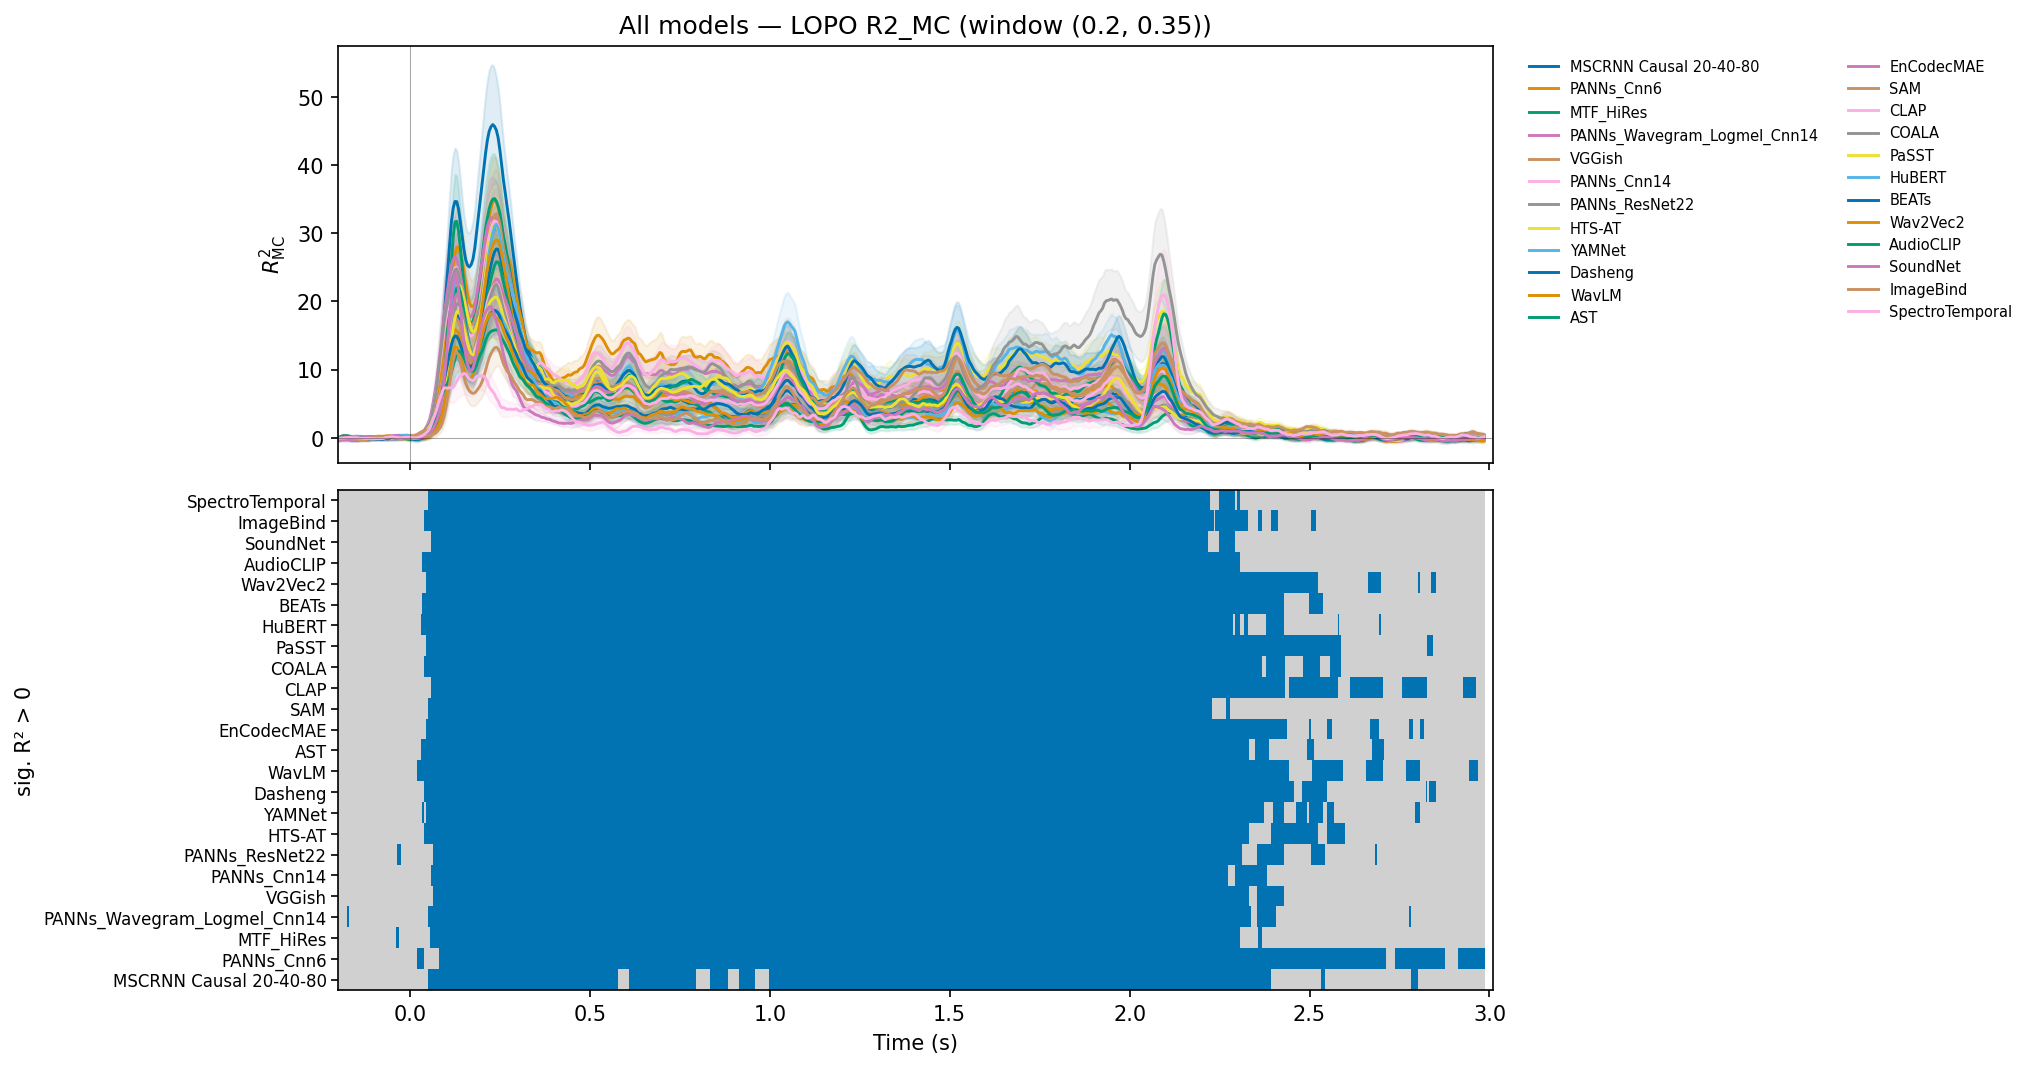
\includegraphics[width=0.95\linewidth]{alignment_curves_all_mc_sig.png}
  \caption{\textbf{Temporal dynamics of brain alignment.} $R^2_{\mathrm{MC}}(t)$ for all models. Shading indicates significant positive alignment. Leading models peak in the 200--500\,ms range.}
  \label{fig:curves}
\end{figure}

\begin{figure}[ht]
  \centering
  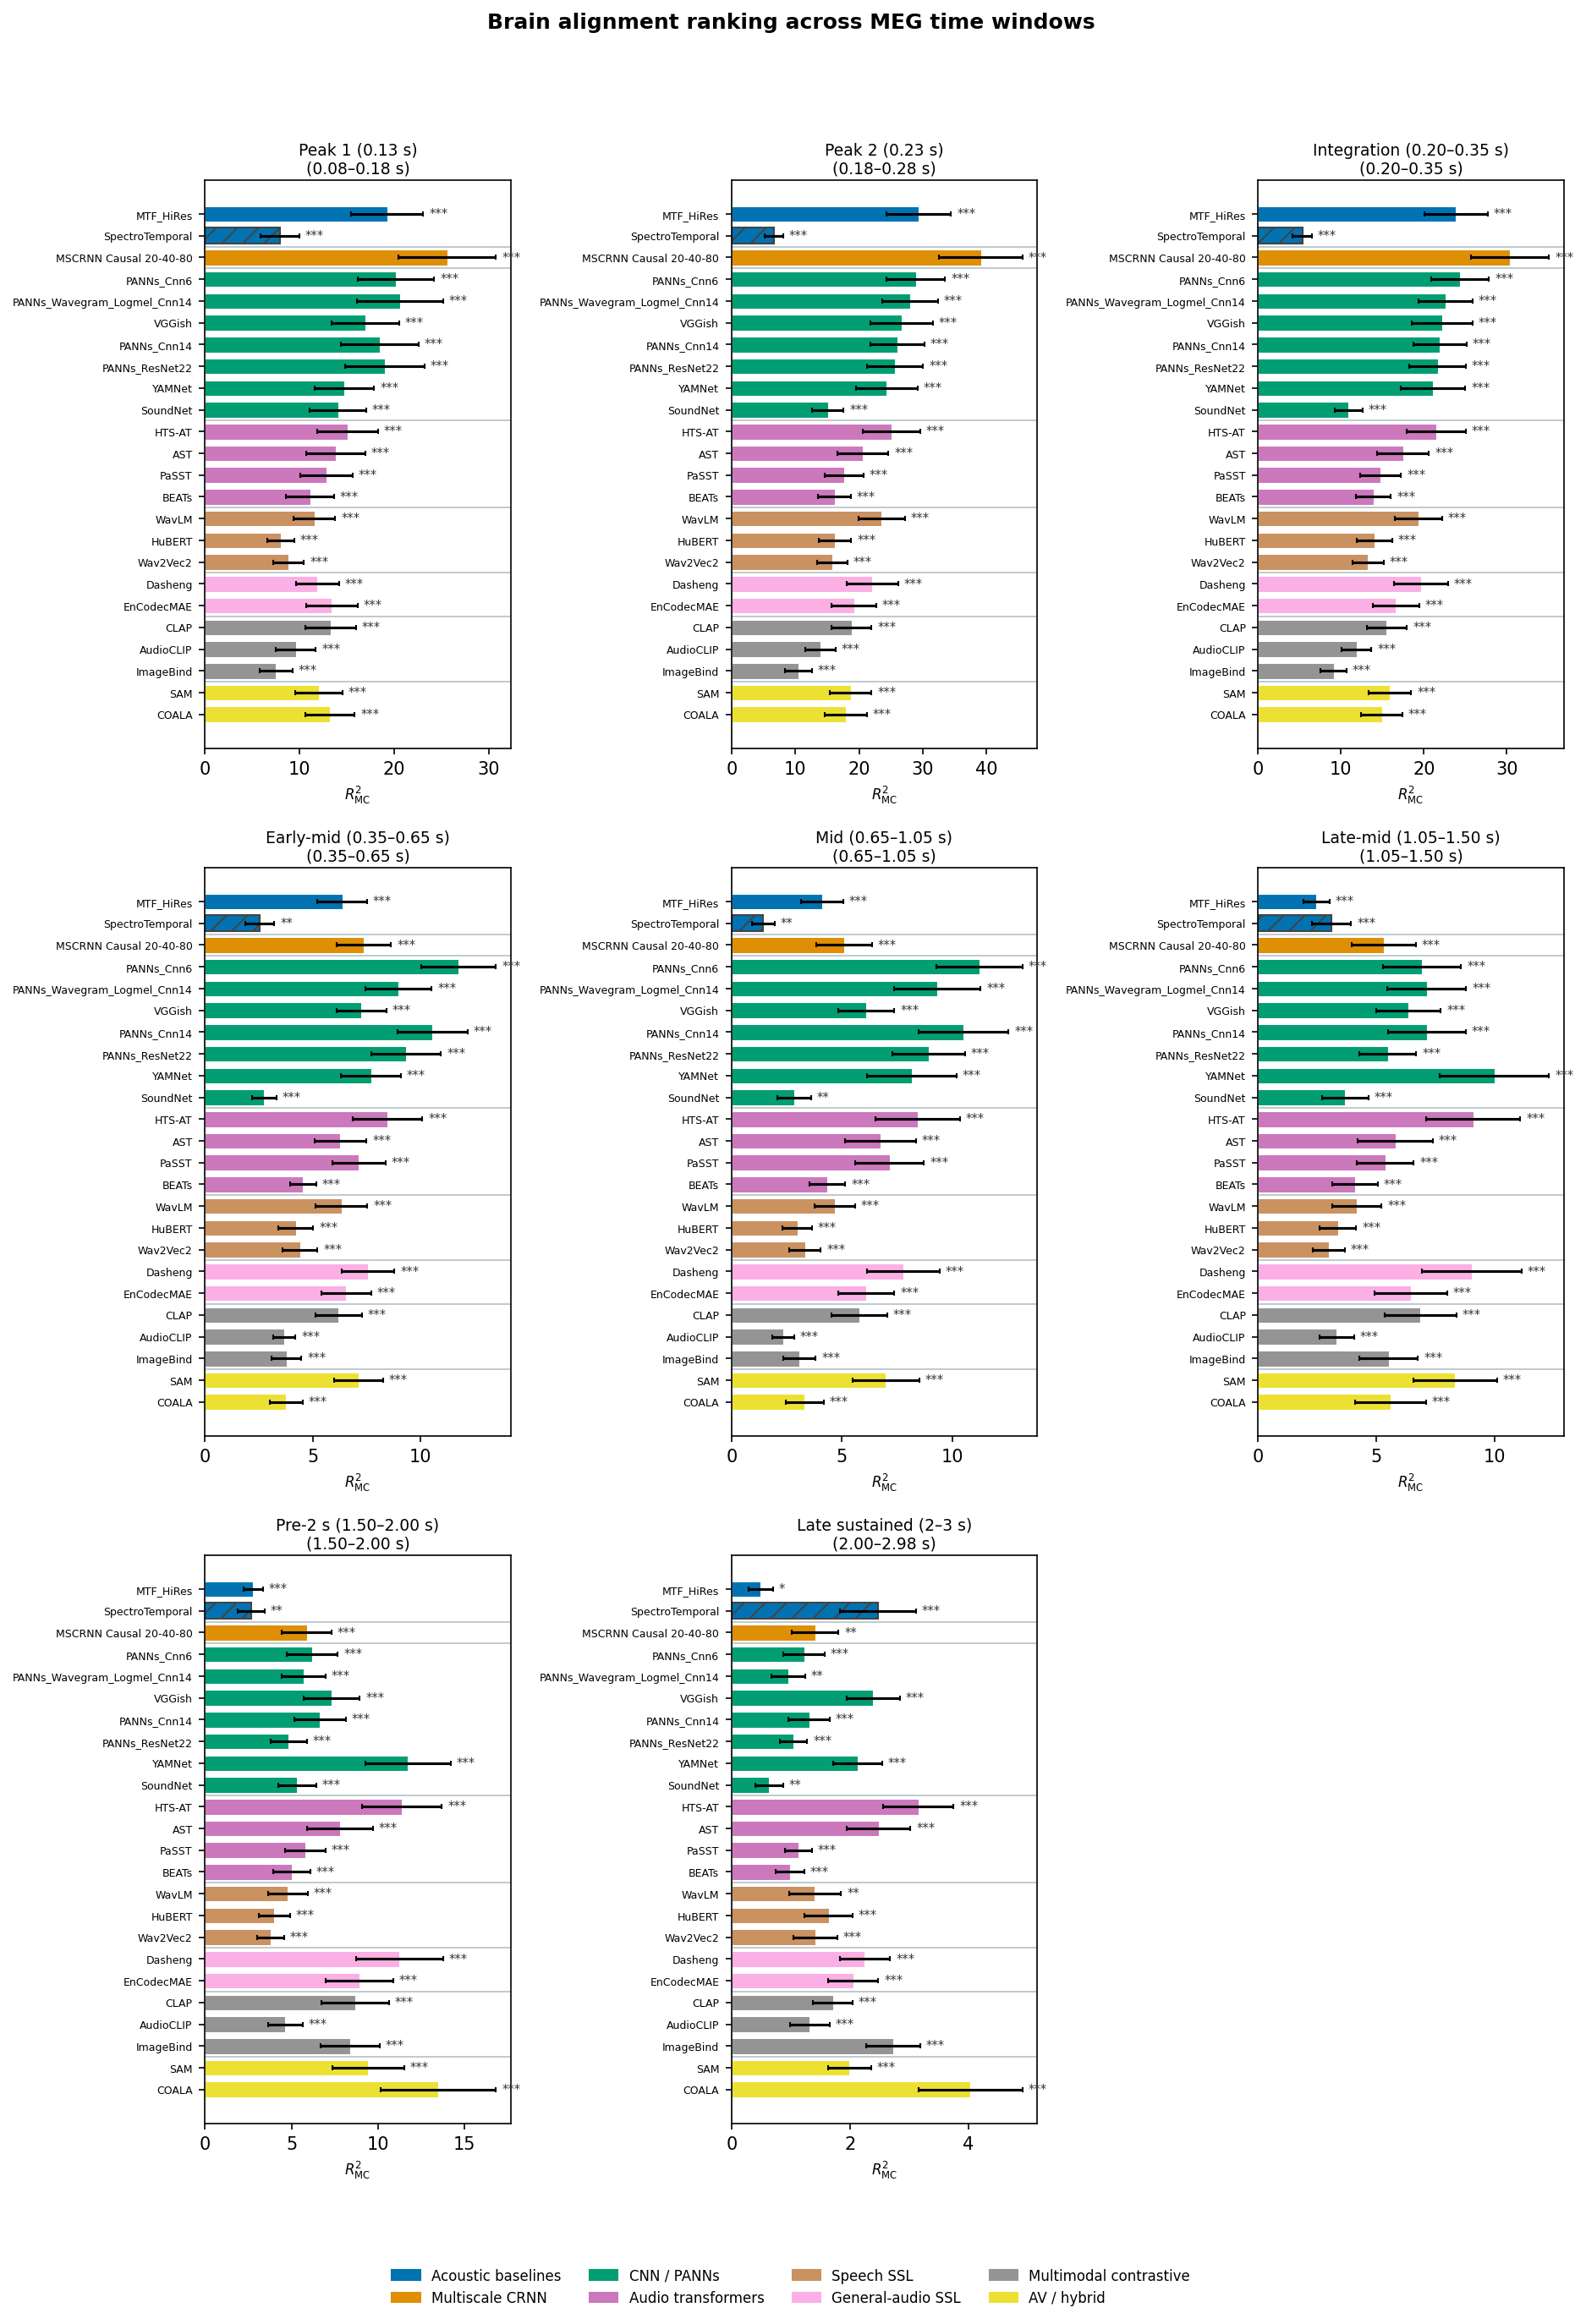
\includegraphics[width=0.95\linewidth]{alignment_scorecard_multi_window.png}
  \caption{\textbf{Multi-window rankings.} Model alignment summarized across five MEG analysis windows. Top ranks are stable across early, integration, and late epochs.}
  \label{fig:scorecard}
\end{figure}

\begin{figure}[ht]
  \centering
  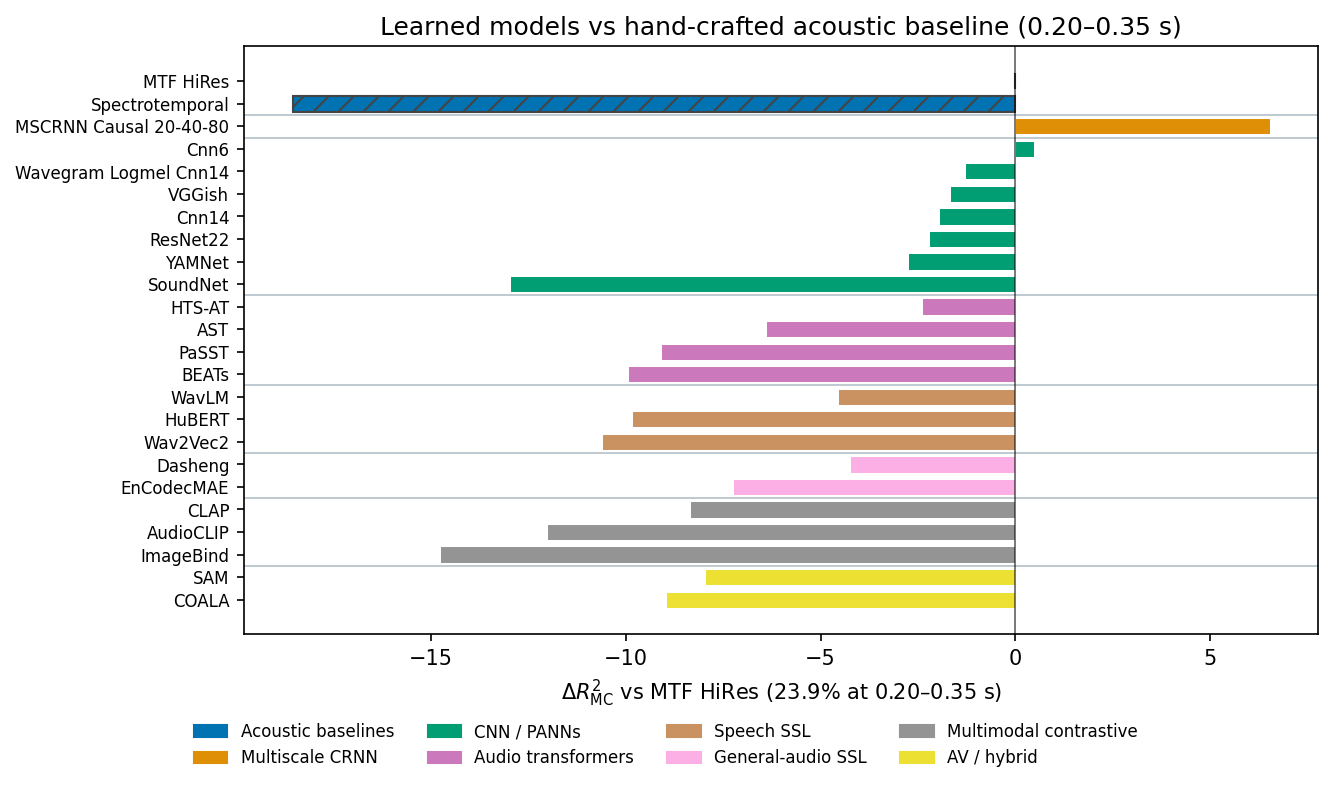
\includegraphics[width=0.92\linewidth]{baseline_lift_vs_mtf_hires.png}
  \caption{\textbf{Gain over an acoustic baseline.} Improvement in $R^2_{\mathrm{MC}}$ relative to the high-resolution MTF model, grouped by architecture family.}
  \label{fig:lift}
\end{figure}

\begin{figure}[ht]
  \centering
  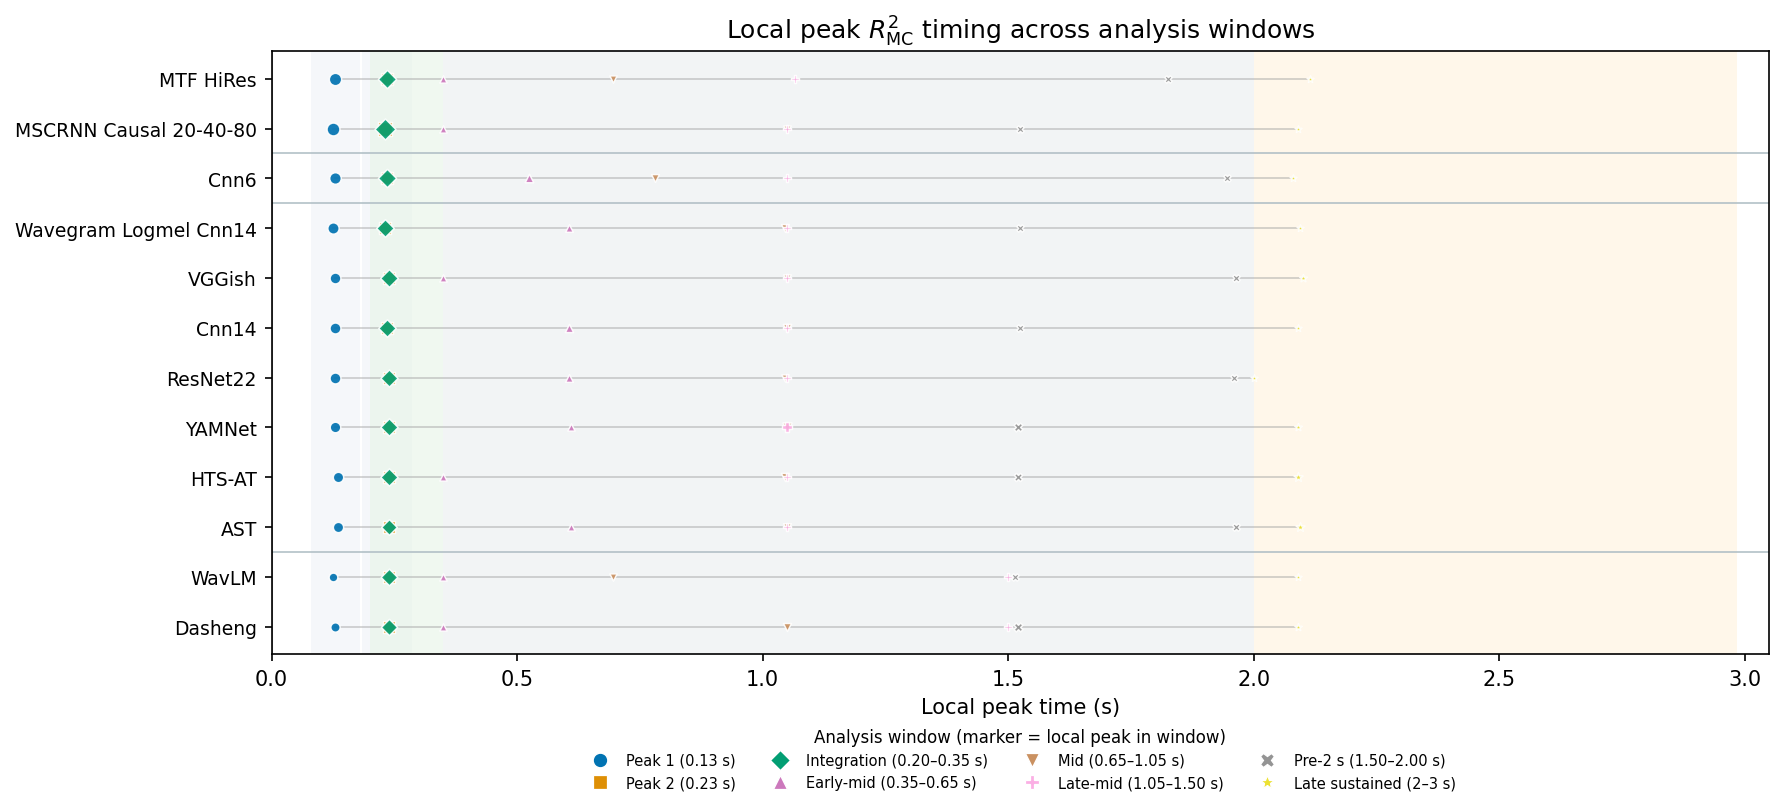
\includegraphics[width=0.92\linewidth]{peak_timing_top12.png}
  \caption{\textbf{When does each model align best?} Peak MEG latency of maximum $R^2_{\mathrm{MC}}$ within each analysis window for the top twelve models.}
  \label{fig:peaktiming}
\end{figure}

\subsection{There is no universal ``brain layer''}

Layer-wise RSA fitted an independent LOPO regression per layer. Peak alignment depth varied markedly across families (Table~\ref{tab:peakdepth}): the recurrent benchmark and MTF model peaked deep in the hierarchy ($\sim$60--68\% normalized depth), whereas speech SSL and some transformers peaked shallow ($\sim$12--17\%). Layer $\times$ time heatmaps (Fig.~\ref{fig:heatmaps}) and multi-window depth profiles (Fig.~\ref{fig:depth}) show that optimal depth is architecture-specific rather than universal.

\begin{table}[ht]
\centering
\caption{Peak brain-aligning layer depth (normalized 0--1) and peak $R^2_{\mathrm{cv}}$.}
\label{tab:peakdepth}
\footnotesize
\begin{tabular}{@{}lrr@{}}
\toprule
\textbf{Model} & \textbf{Peak depth} & \textbf{Peak $R^2_{\mathrm{cv}}$} \\
\midrule
MSCRNN Causal 20-40-80 & 0.68 & 0.0064 \\
MTF\_HiRes & 0.61 & 0.0061 \\
CLAP & 0.17 & 0.0051 \\
Dasheng & 0.53 & 0.0047 \\
WavLM & 0.12 & 0.0046 \\
PANNs\_Cnn6 & 0.25 & 0.0043 \\
BEATs & 0.16 & 0.0040 \\
\bottomrule
\end{tabular}
\end{table}

\begin{figure}[ht]
  \centering
  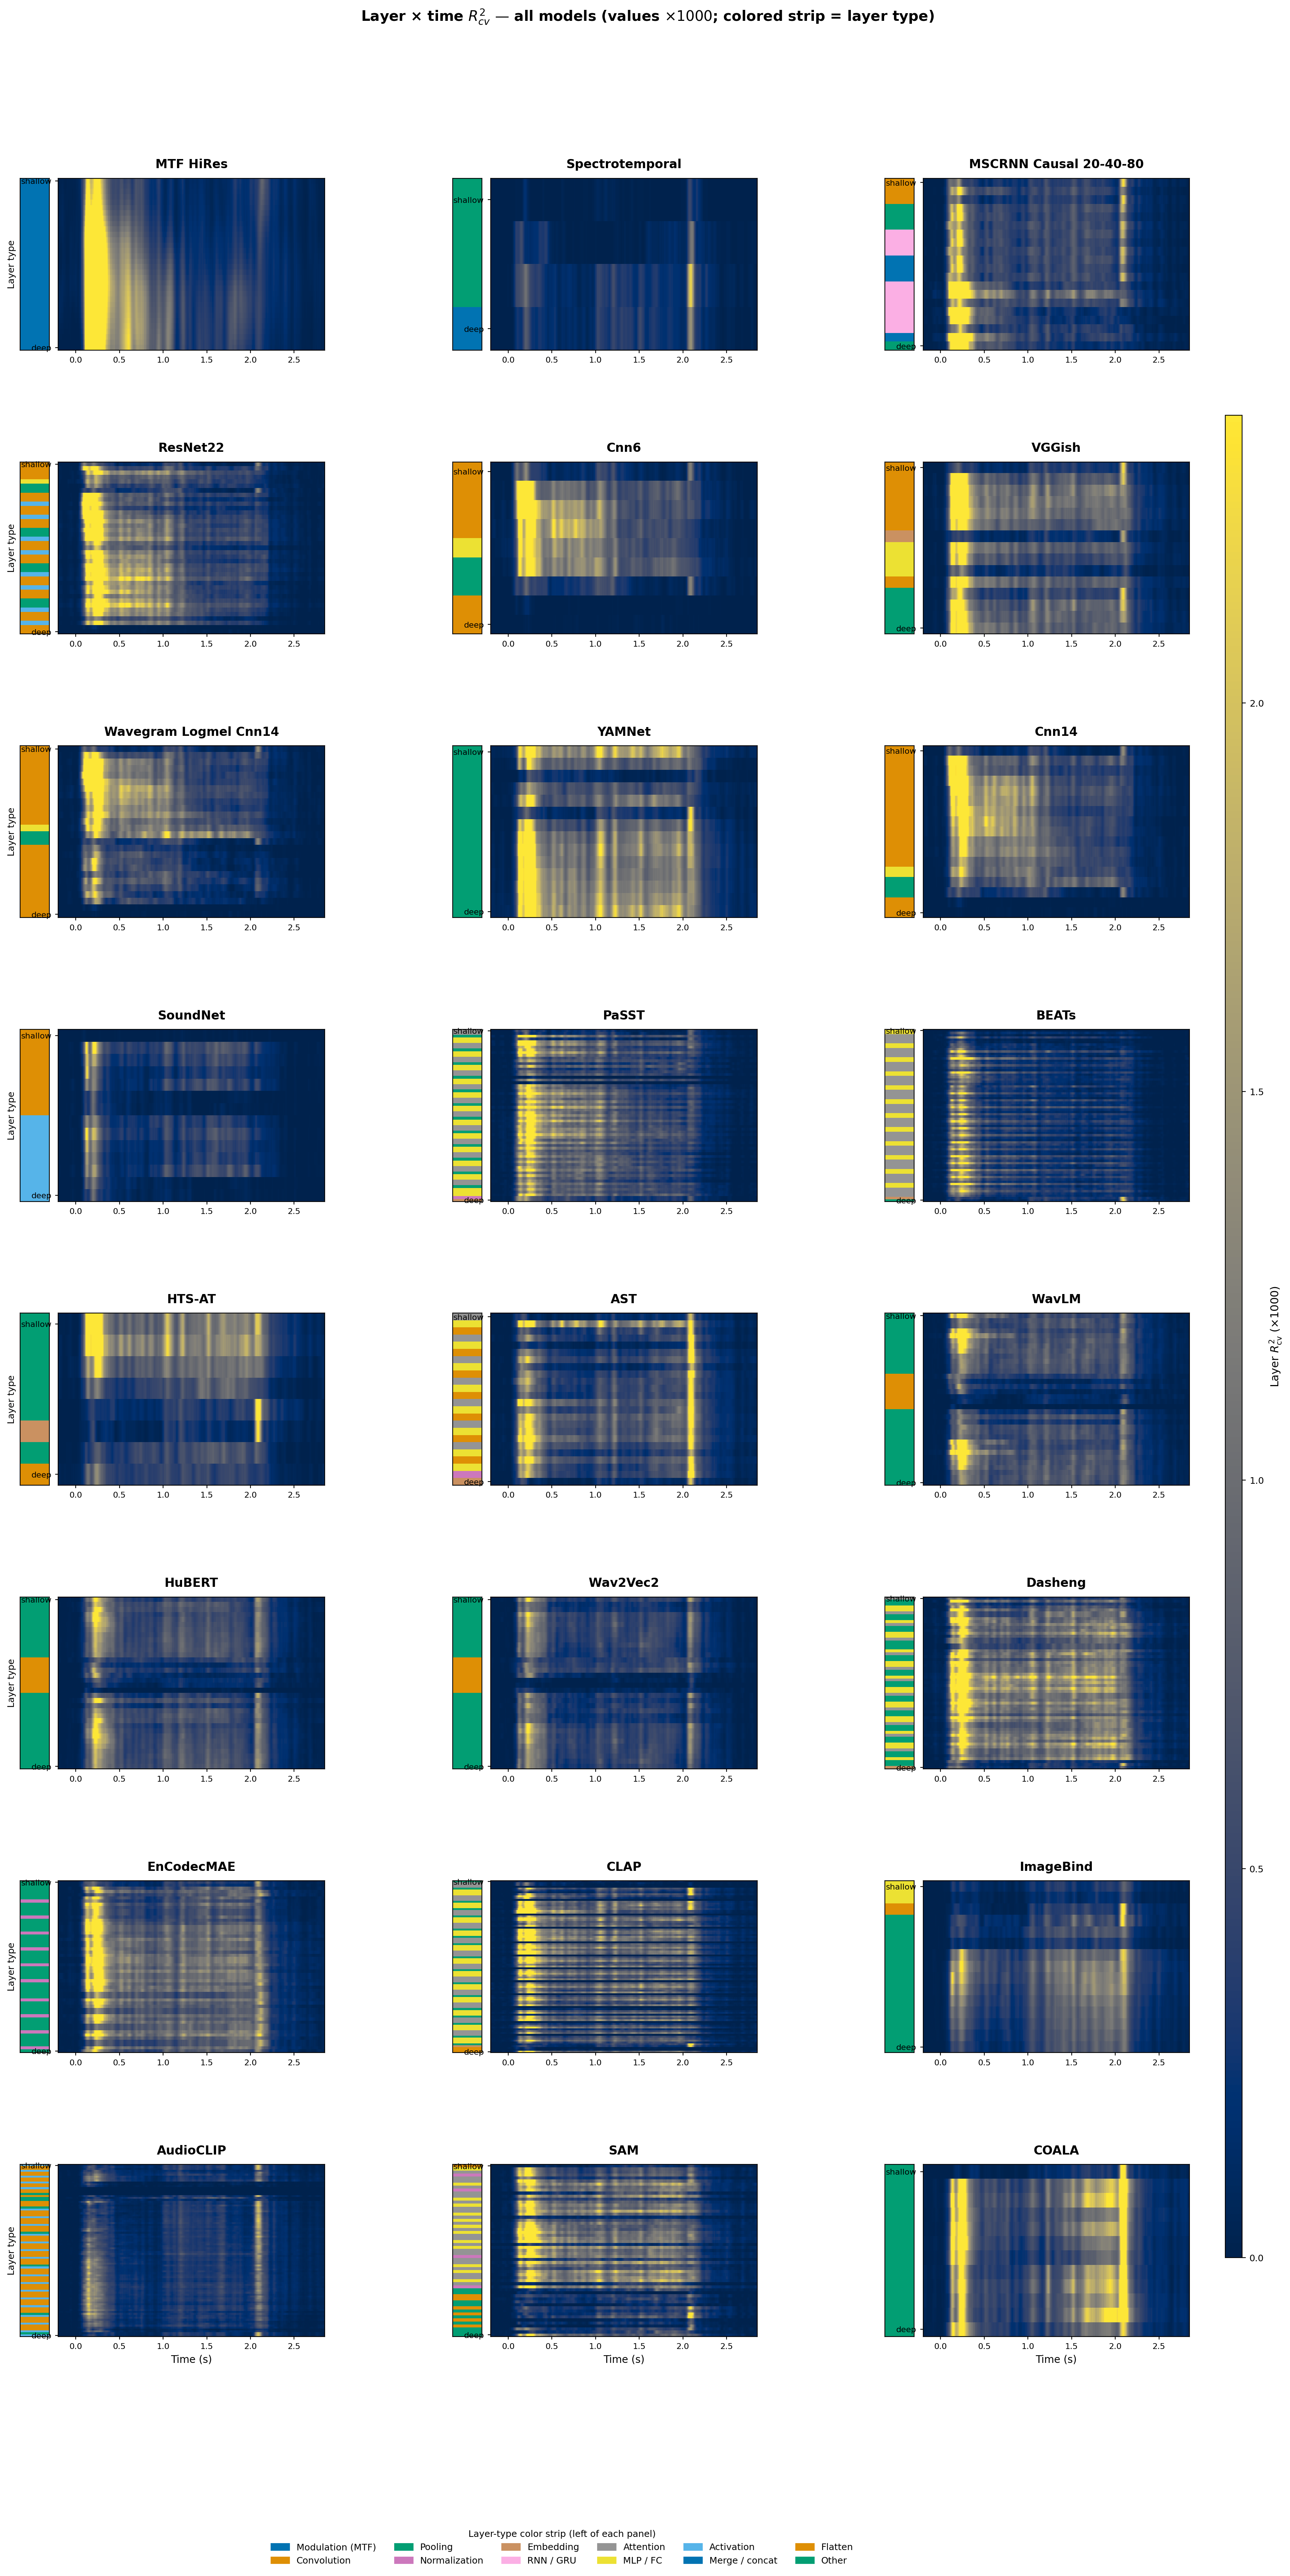
\includegraphics[width=0.95\linewidth]{layer_heatmap_grid_all_models.png}
  \caption{\textbf{Layer $\times$ time landscapes.} Brain alignment ($R^2_{\mathrm{cv}}$) across depth and MEG time for all DNNs. Alignment patterns differ qualitatively across families.}
  \label{fig:heatmaps}
\end{figure}

\begin{figure}[ht]
  \centering
  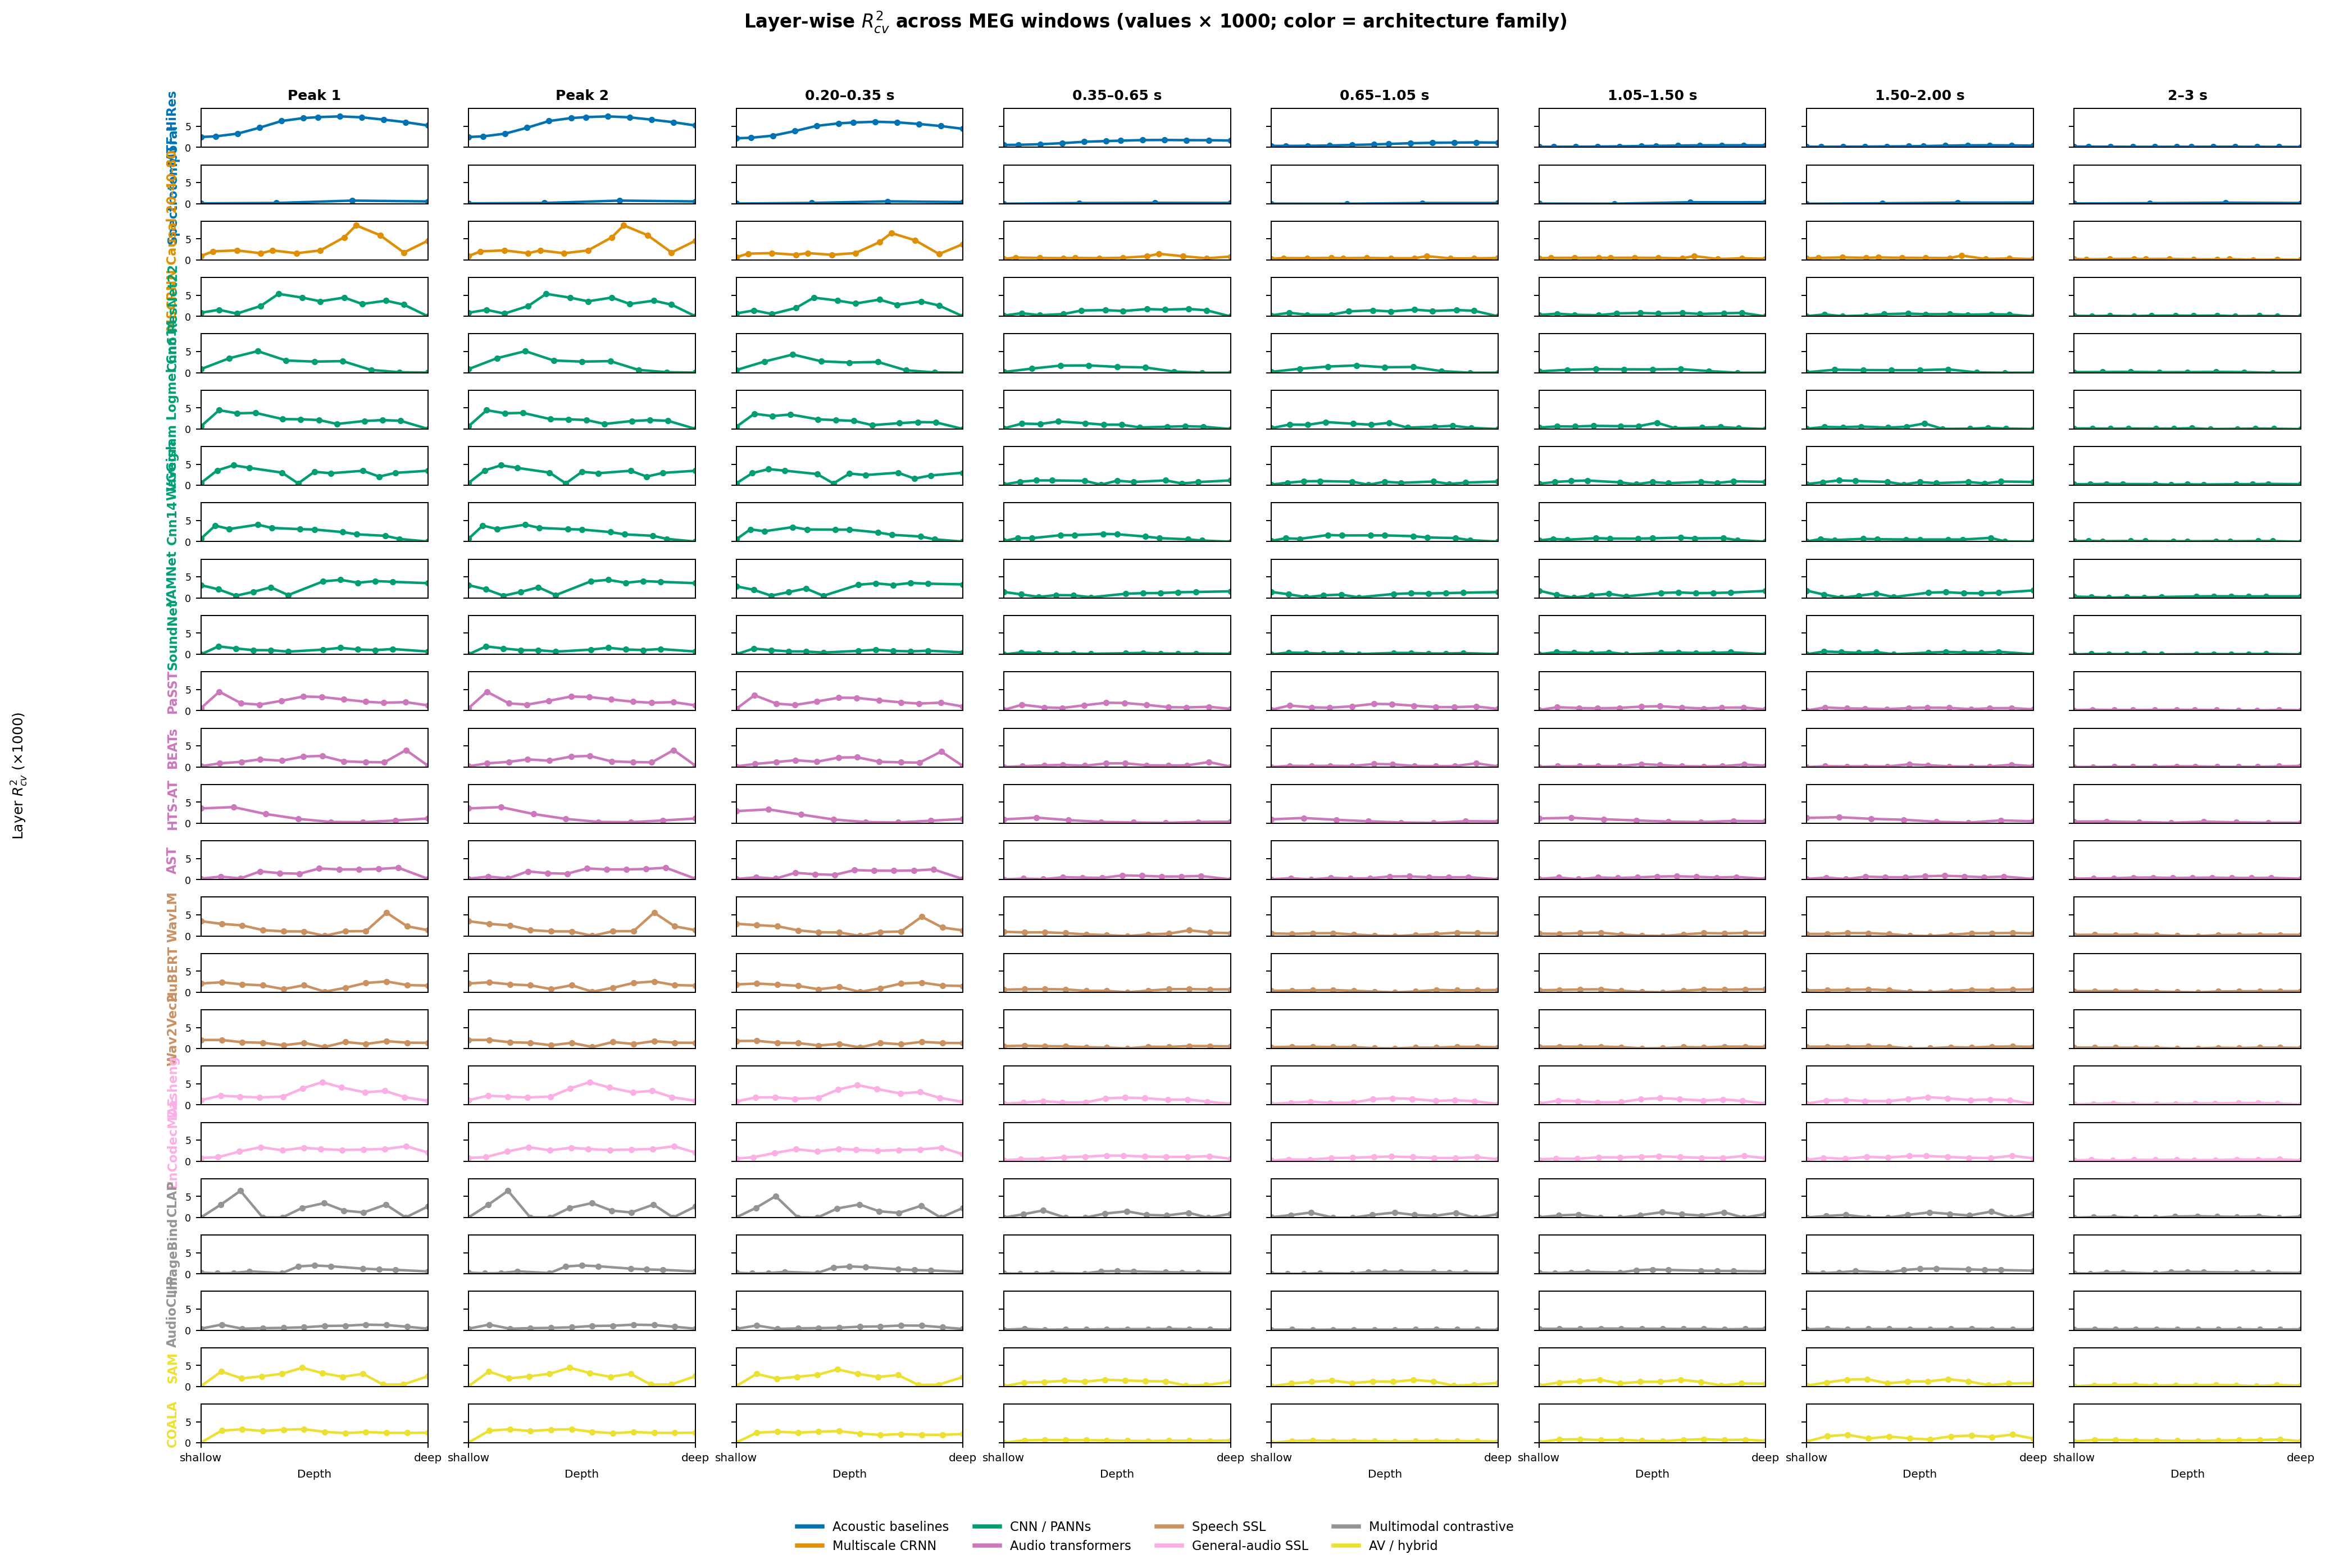
\includegraphics[width=0.95\linewidth]{layer_depth_multiwindow_all_models.png}
  \caption{\textbf{Depth profiles across MEG windows.} Normalized layer depth of peak alignment, color-coded by architecture family.}
  \label{fig:depth}
\end{figure}

\subsection{Training objective explains \emph{which network} aligns; layer class explains \emph{which layer}}

To move beyond descriptive rankings, we regressed layer-wise alignment strength against architectural metadata ($n=784$ DNN layers; acoustic baselines and the recurrent benchmark excluded due to non-comparable layer structure). Univariate models (Table~\ref{tab:uni_primary}) showed that training objective and architecture family carry the largest marginal explanatory power across all layers.

\begin{table}[ht]
\centering
\caption{Marginal $R^2$ for single-factor models predicting layer-wise alignment ($n=784$ layers).}
\label{tab:uni_primary}
\footnotesize
\begin{tabular}{@{}lr@{}}
\toprule
\textbf{Factor} & \textbf{$R^2_{\mathrm{univ}}$} \\
\midrule
Training objective & 0.23 \\
Architecture family & 0.15 \\
Training modality & 0.11 \\
Layer class (conv / attention / MLP / embed) & 0.10 \\
Input representation & 0.04 \\
\bottomrule
\end{tabular}
\end{table}

Split-level analysis separated \emph{between-network} from \emph{within-network} questions. Between models ($n=21$ network means), training objective explained 75\% of variance, architecture family 55\%, and training modality 50\%. Within models ($n=784$ layer deviations from network means), layer class explained only 6\%; depth explained almost nothing. In short: choosing the network matters far more than choosing a depth within it.

A three-way variance partition (architecture family $\times$ training objective $\times$ layer class) attributed 31\% of total variance to the joint model and 69\% to unexplained sources (Fig.~\ref{fig:varpart}). Unique contributions were modest: layer class 6.3\%, training objective 5.0\%, architecture family 3.3\%. Multi-window regression confirmed that training objective and architecture family dominate across MEG epochs (Fig.~\ref{fig:varpart_windows}).

Treating peak MEG latency as an outcome, training objective explained 72\% of between-model variance in \emph{when} layers align best. Linear mixed models with random intercepts per network confirmed that MLP/fully-connected layers align more strongly than embeddings ($p=0.002$), and multimodal training objectives align less well than unimodal audio training ($p<0.001$).

\begin{figure}[ht]
  \centering
  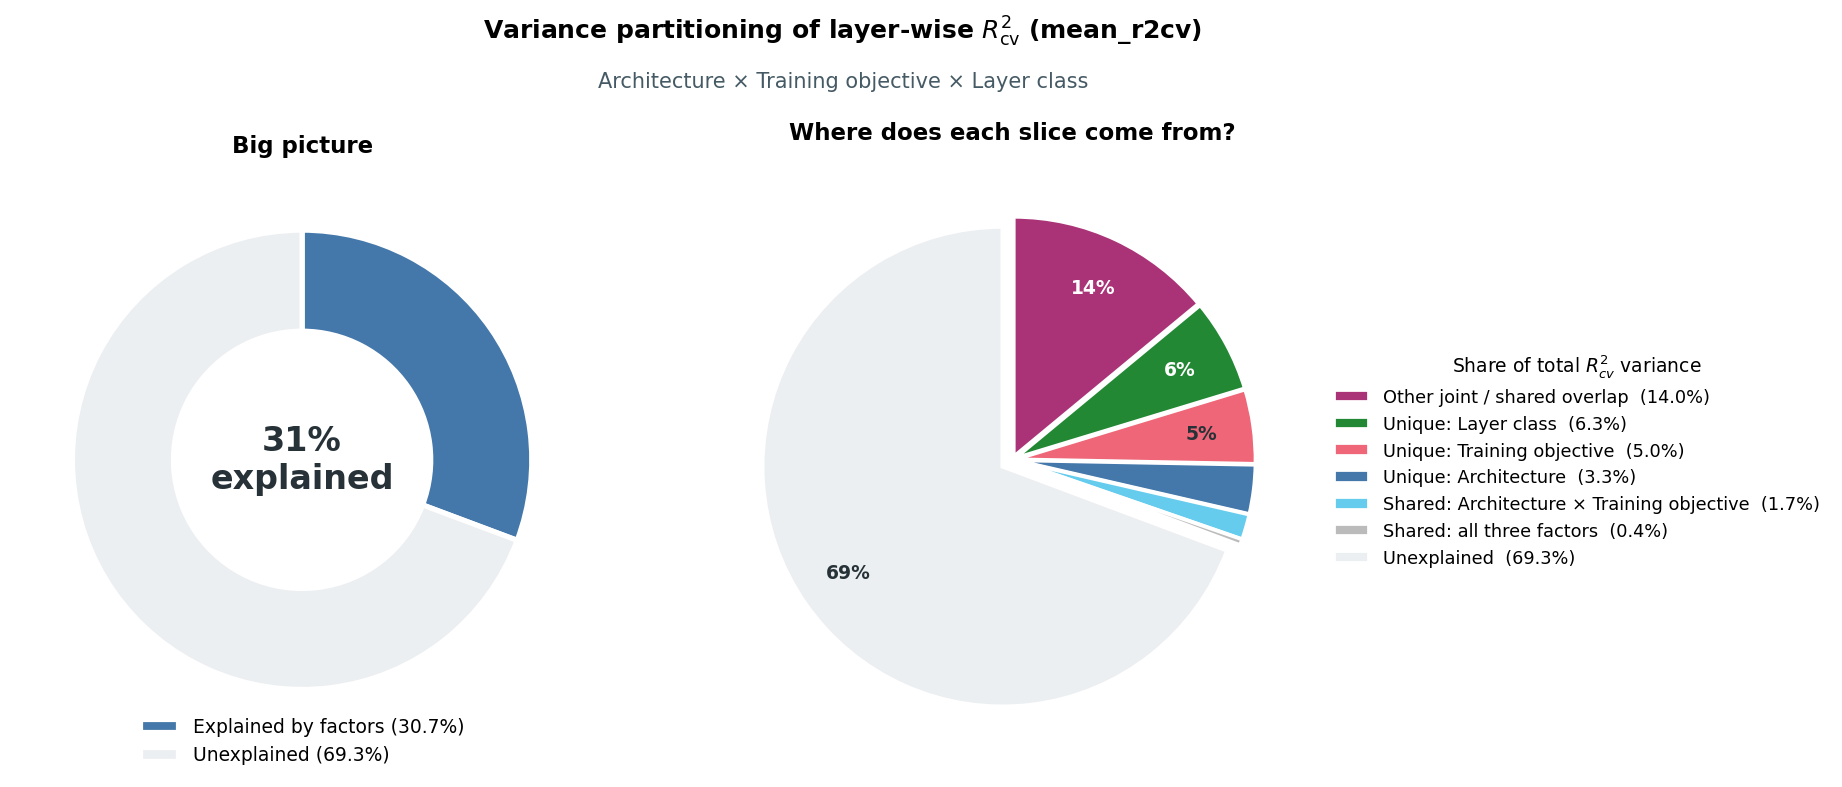
\includegraphics[width=0.95\linewidth]{variance_decomposition_main.png}
  \caption{\textbf{What explains layer-wise alignment?} Variance partition of $R^2_{\mathrm{cv}}$ across architecture family, training objective, and layer class. Only $\sim$31\% of variance is jointly explained; most remains unexplained.}
  \label{fig:varpart}
\end{figure}

\begin{figure}[ht]
  \centering
  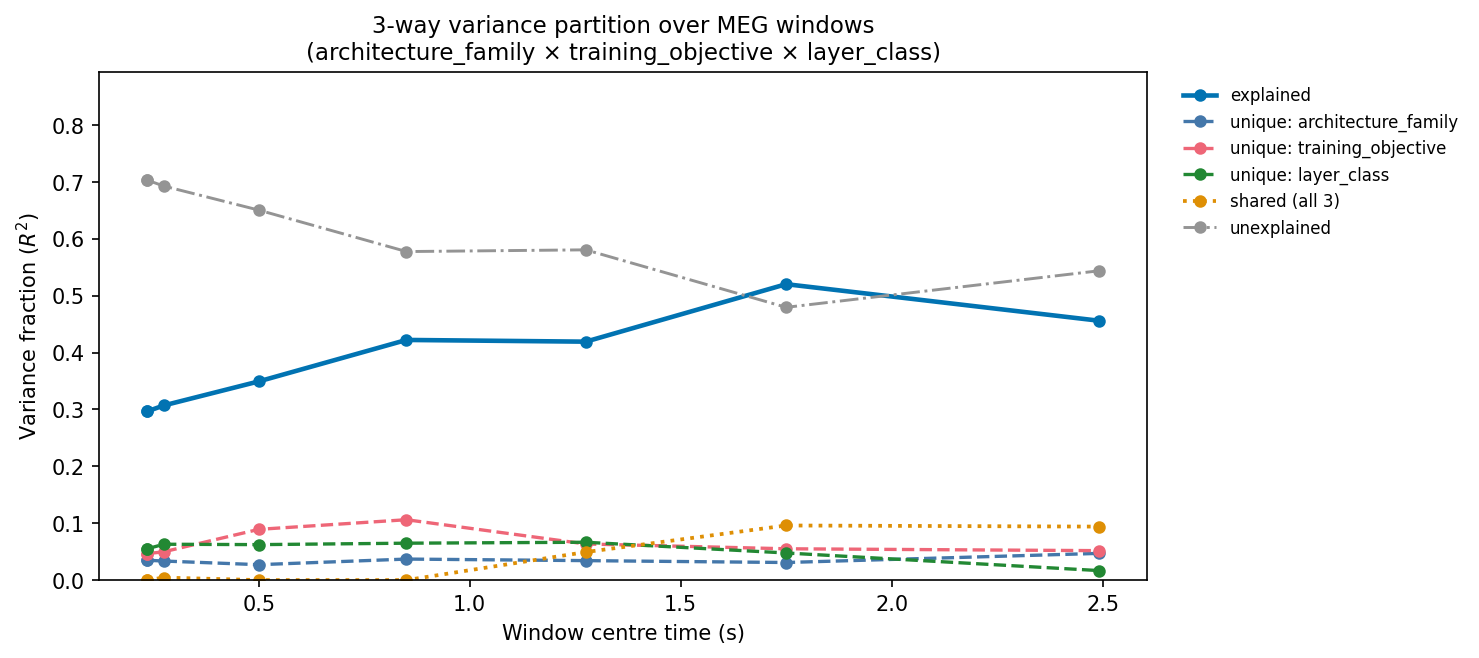
\includegraphics[width=0.95\linewidth]{variance_partition_venn_over_windows.png}
  \caption{\textbf{Variance components across MEG windows.} Explained fractions for the three-way partition recomputed at each analysis epoch.}
  \label{fig:varpart_windows}
\end{figure}

\subsection{fMRI: early auditory cortex aligns; higher ROIs collapse toward null}

To test whether MEG-favoured models remain brain-like beyond sensor averages, we applied the same Sound-DNN zoo to auditory fMRI betas (reliability-selected voxels in Glasser parcels; common 150 sounds shared across participants). Predictive RSA used Euclidean brain RDMs, cosine model predictors, theoretical RDM whitening matched to the MEG pipeline, leave-one-participant-out cross-validation, and group-scope Monte-Carlo standardization ($R^2_{\mathrm{MC}}$; Gaussian synthetic-brain nulls).

In primary auditory cortex (A1), all 31 evaluated models showed positive median $R^2_{\mathrm{MC}}$ (Fig.~\ref{fig:fmri_a1}). The A1 leaderboard was led by EnCodecMAE (median $R^2_{\mathrm{MC}}=761$), COALA ($590$), and the Aud2Sem categorical DNN ($246$), with acoustic references (AudDims, SpectroTemporal, MTF variants) and the causal MSCRNN also strongly above null. Spearman rank correlation between raw LOPO $R^2_{\mathrm{cv}}$ and $R^2_{\mathrm{MC}}$ was high ($\rho=0.97$), indicating that MC standardization reshapes magnitudes more than order.

Across the anatomical hierarchy (Fig.~\ref{fig:fmri_hierarchy}--\ref{fig:fmri_traj}), mean model $R^2_{\mathrm{MC}}$ remained strongly positive in Heschl's gyrus / early auditory belts (A1, LBelt, MBelt, PBelt, TA2) and dorsal STG (A4), weakened in A5, and collapsed toward or below null in STGa, STS parcels, insula, and frontal language-adjacent ROIs (Area~44/45, IFJ). STS demeaning and whitening variants did not rescue alignment. Thus fMRI reveals a clear early-auditory focus of current audio DNNs that MEG sensor RSA---which mixes sources---cannot localize.

\begin{figure}[ht]
  \centering
  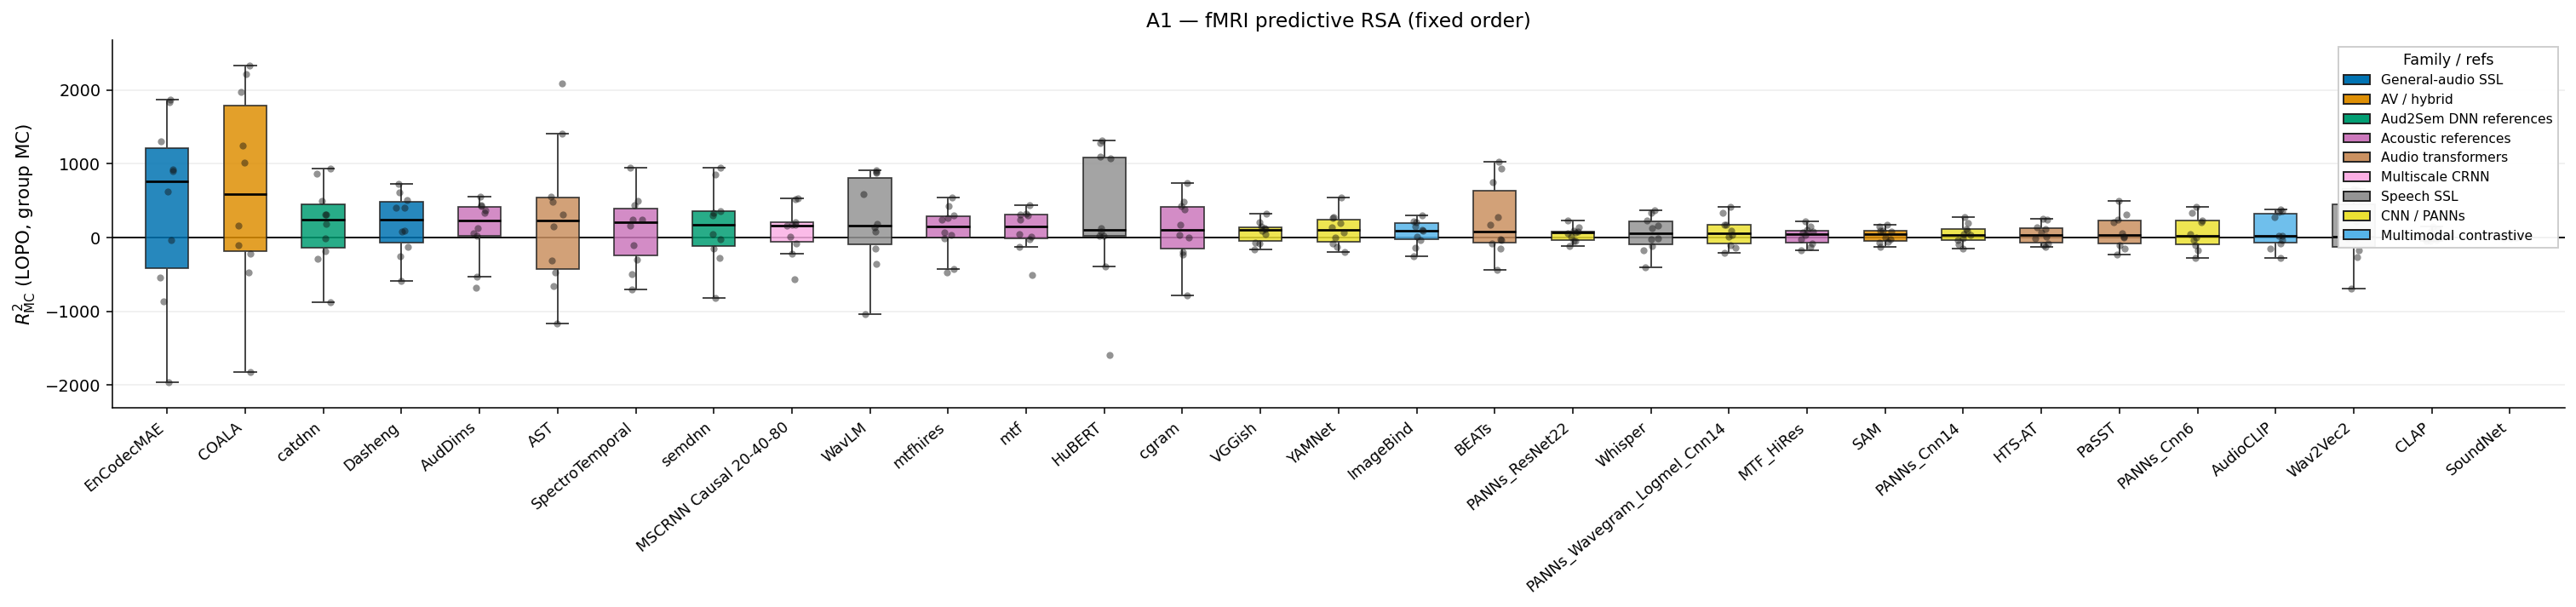
\includegraphics[width=0.95\linewidth]{fmri_rsa_mc_A1.png}
  \caption{\textbf{fMRI A1 leaderboard ($R^2_{\mathrm{MC}}$).} Leave-one-participant-out predictive RSA on Glasser A1 betas (common 150 sounds; nodemean + theoretical whitening). Boxes show subject-wise $R^2_{\mathrm{MC}}$; models ordered by A1 median.}
  \label{fig:fmri_a1}
\end{figure}

\begin{figure}[ht]
  \centering
  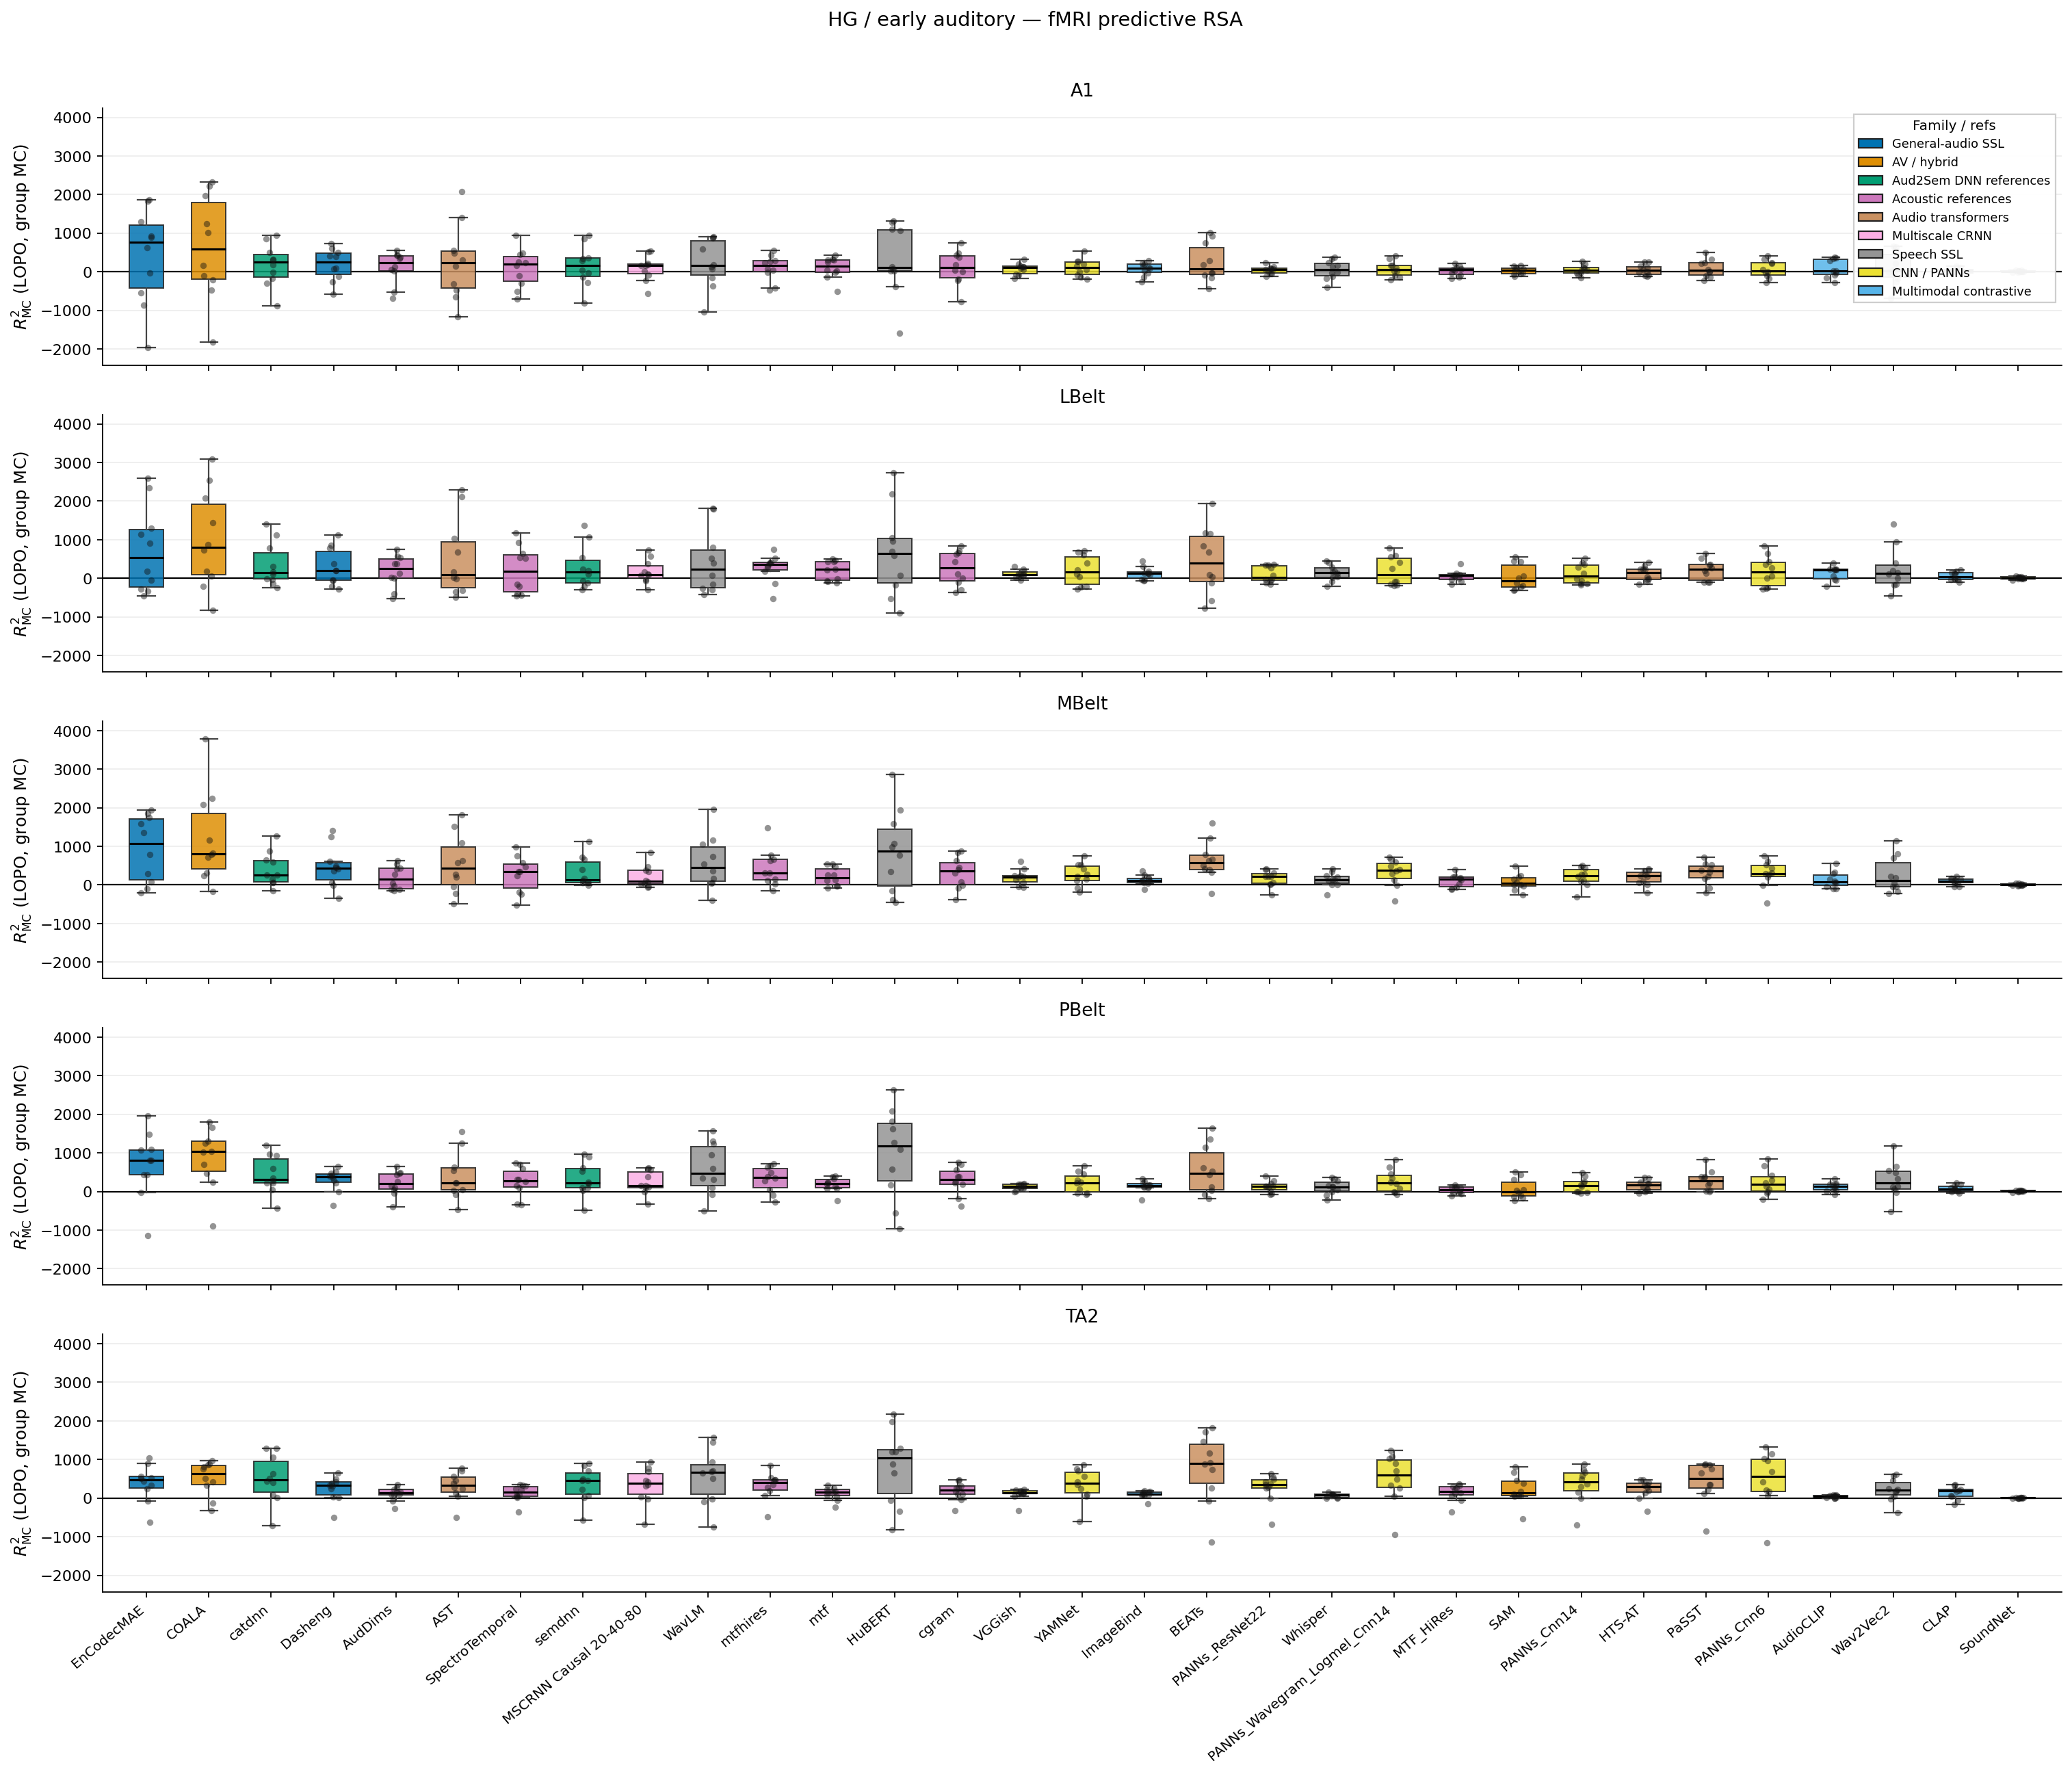
\includegraphics[width=0.95\linewidth]{fmri_rsa_mc_hg_early.png}
  \caption{\textbf{Early auditory fMRI hierarchy.} $R^2_{\mathrm{MC}}$ for HG / early auditory parcels (A1, LBelt, MBelt, PBelt, TA2) with model order frozen from A1.}
  \label{fig:fmri_hierarchy}
\end{figure}

\begin{figure}[ht]
  \centering
  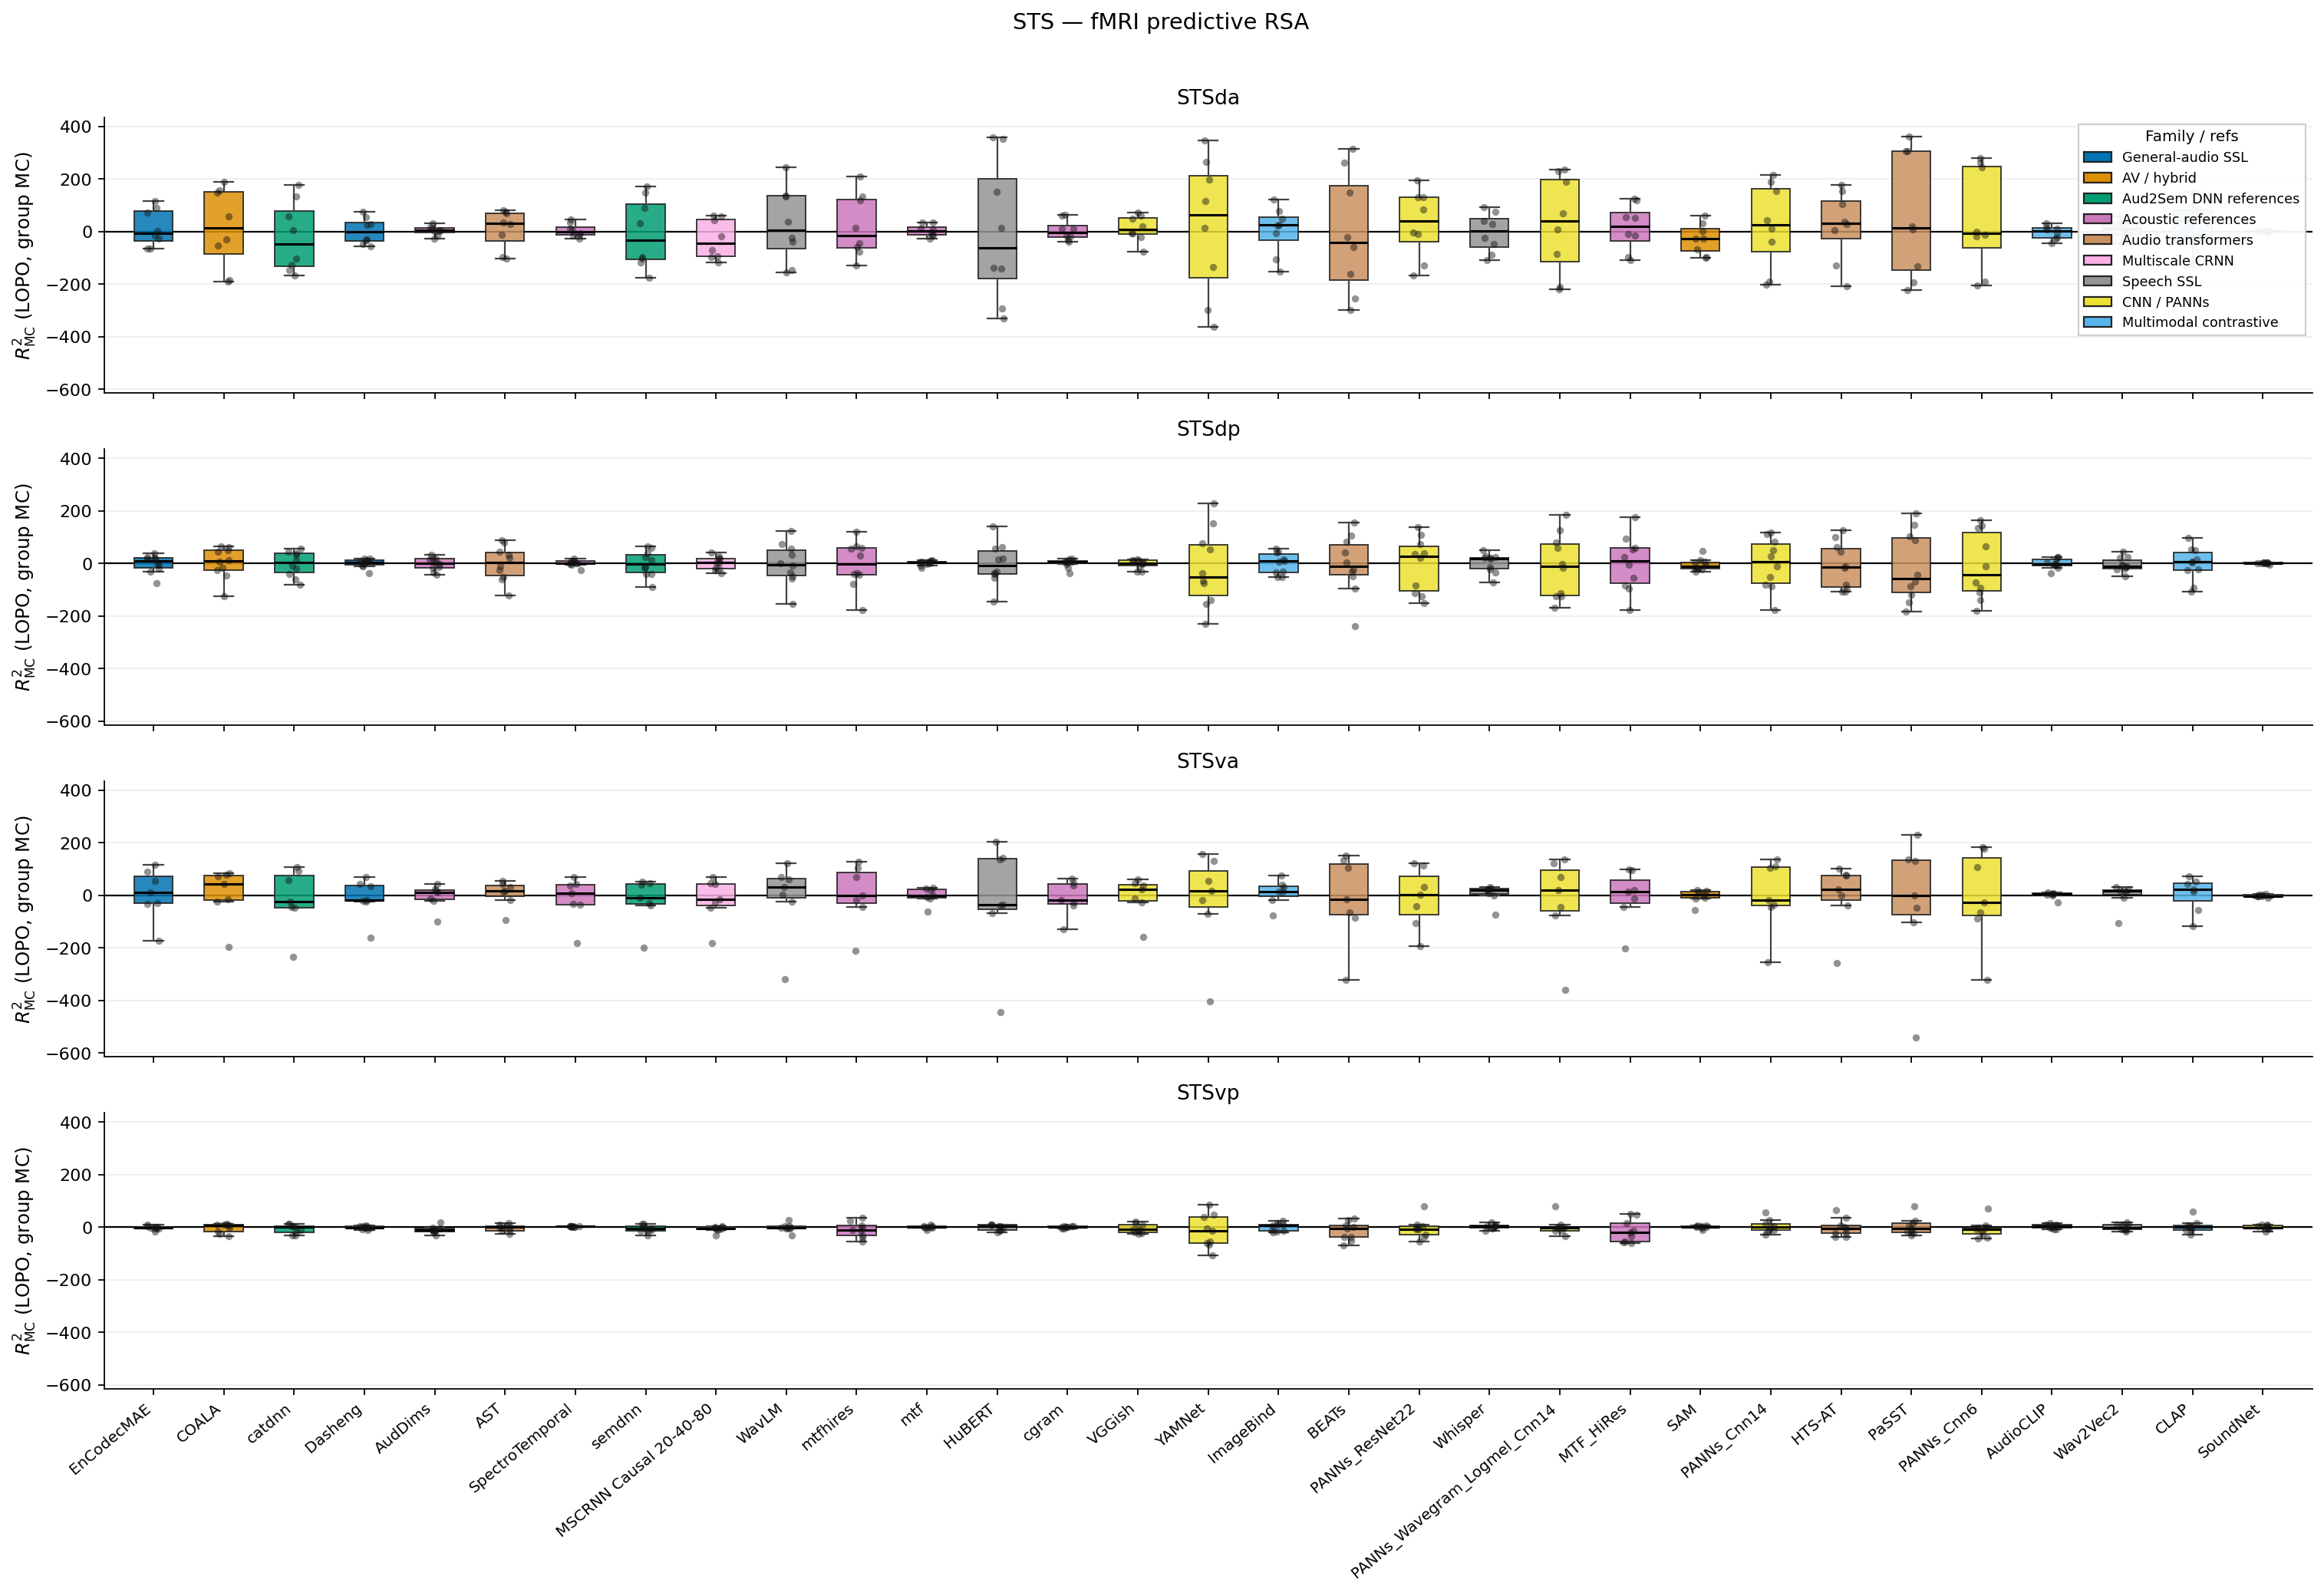
\includegraphics[width=0.92\linewidth]{fmri_rsa_mc_sts.png}
  \caption{\textbf{STS fMRI alignment near null.} Same analysis as Fig.~\ref{fig:fmri_hierarchy} for STSda/dp/va/vp; medians hug zero across the model zoo.}
  \label{fig:fmri_sts}
\end{figure}

\begin{figure}[ht]
  \centering
  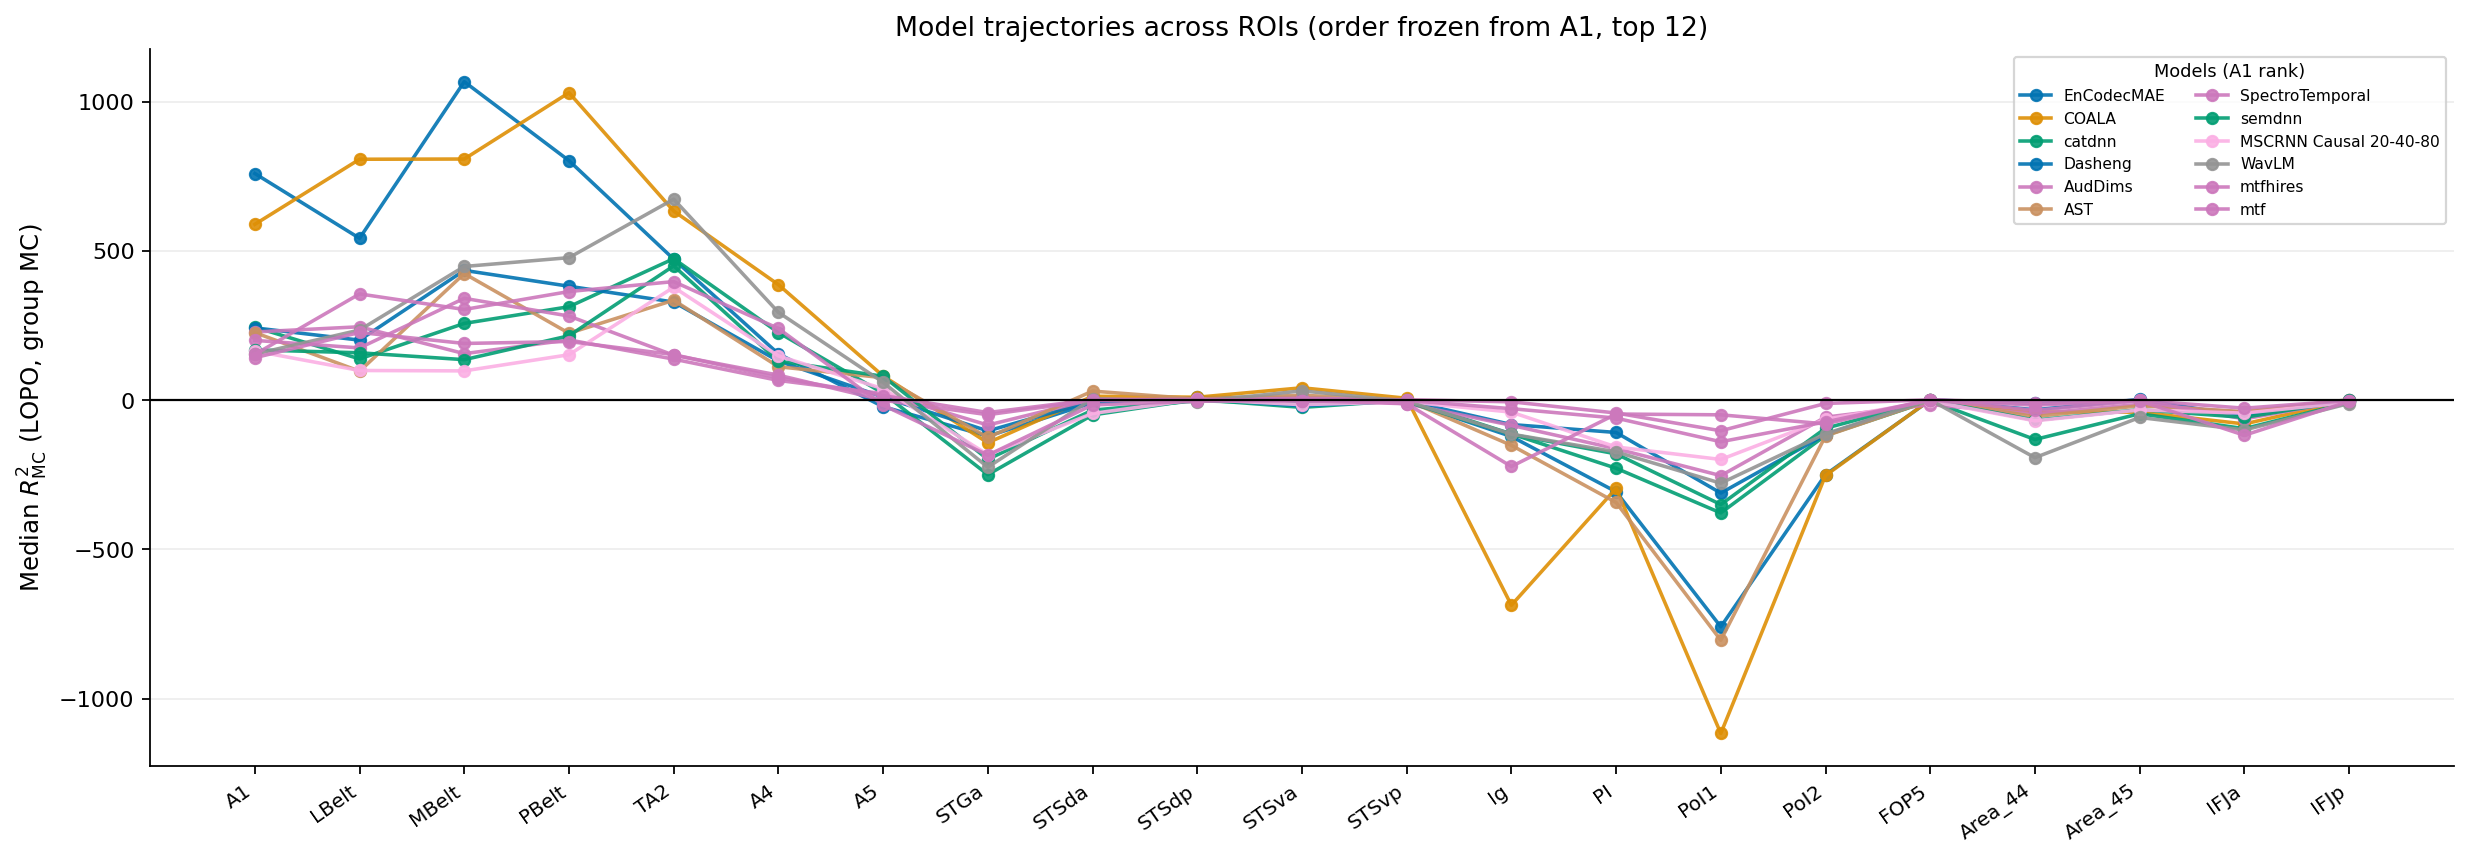
\includegraphics[width=0.95\linewidth]{fmri_rsa_mc_trajectories.png}
  \caption{\textbf{Model trajectories across Glasser ROIs.} Top-12 A1 models tracked from early auditory cortex through STG, STS, insula, and frontal parcels ($R^2_{\mathrm{MC}}$).}
  \label{fig:fmri_traj}
\end{figure}

\section{Discussion}

Four conclusions emerge. \textbf{First}, brain alignment in MEG sensor-space RSA is not monotonic with model size, recency, or general-audio leaderboard rank. Compact supervised CNNs and hand-crafted spectrotemporal features rival or exceed large SSL transformers. The success of the causal recurrent benchmark underscores that architectures explicitly optimized for temporally structured acoustic input can capture variance in human MEG that general-purpose encoders miss at the sensor level.

\textbf{Second}, there is no single ``brain layer.'' Optimal depth depends on model genealogy and training objective; shallow speech SSL layers and deep recurrent stages can both win, but for different networks. \textbf{Third}, variance-partition regression formalizes a distinction often blurred in the literature: between-network differences are driven mainly by training objective and architecture family, whereas within-network layer rankings are only weakly structured by block type.

\textbf{Fourth}, fMRI ROI RSA shows that the same model zoo is strongly brain-like in early auditory cortex yet largely fails in STS, insula, and frontal parcels. MEG and fMRI therefore answer complementary questions: MEG ranks \emph{when} and \emph{how strongly} models match population geometry in time; fMRI ranks \emph{where} along cortex that match survives. Bridging the two---and extending source-localized MEG to Destrieux / Glasser macros---is a priority for the next iteration of this benchmark.

\subsection{Limitations}

MEG analyses were performed in sensor space; source-localized RSA may reorder models. Leaderboard $R^2_{\mathrm{MC}}$ values are standardized effect sizes, not variance explained; layer-wise $R^2_{\mathrm{cv}}$ operates on a much smaller absolute scale ($\sim$0.001--0.006). All DNN embeddings were evaluated with a harmonized two-window temporal pooling scheme, which may disadvantage architectures with fixed single-window inputs. Architectural metadata were assigned from published descriptions and require independent verification before publication. fMRI used Euclidean RDMs on condition-averaged betas (no trial-level crossnobis) and Gaussian synthetic-brain Monte-Carlo nulls; subject counts vary by ROI as reliability-selected voxel masks shrink outside early auditory cortex. Maastricht Glasser parcels are not one-to-one with MEG macro-ROI atlases.

\section{Methods}

\subsection{Participants and stimuli}
Twenty-one healthy participants passively listened to natural sounds in the Aud2Sem MEG paradigm. Stimuli comprised 600 RMS-normalized natural sounds drawn from FSD50K-derived sets, organized into one common and three participant-unique splits of 150 sounds each for LOPO cross-validation. A silence trial was excluded from RSA. Semantic labels and cluster metadata accompanied each sound.

\subsection{MEG preprocessing and brain RDMs}
Sensor-level crossnobis RDMs were computed with Ledoit--Wolf covariance estimation, cross-validated leave-one-out partitioning, 200\,Hz resampling, and 40\,ms temporal bins. RDMs were whitened and z-scored prior to RSA.

\subsection{Representational models}
Twenty-four models spanned supervised CNNs (PANNs family, VGGish, YAMNet, SoundNet), audio transformers (AST, PaSST, HTS-AT, BEATs), speech SSL (Wav2Vec2, HuBERT, WavLM), general-audio SSL (Dasheng, EnCodecMAE), multimodal contrastive encoders (CLAP, AudioCLIP, ImageBind, COALA, SAM/PE-AV), acoustic baselines (high-resolution MTF, spectrotemporal mel proxy), and a causal multiscale recurrent benchmark (MSCRNN). All DNNs were used in inference mode with publicly available pre-trained weights; no fine-tuning on the stimulus set. Table~\ref{tab:modelzoo} lists architecture family, evaluation tier, sampling rate, and layer count.

% Model zoo table (included from main.tex). Reference column: fill in references.bib.
\begin{longtable}{@{}p{3.2cm}lllrp{2.2cm}@{}}
\caption{Representational models included in the benchmark. Primary reference per model: [TBD].}
\label{tab:modelzoo} \\
\toprule
\textbf{Model} & \textbf{Family} & \textbf{Tier} & \textbf{SR} & \textbf{L} & \textbf{Ref.} \\
\midrule
\endfirsthead
\multicolumn{6}{c}{\textit{(continued)}} \\
\toprule
\textbf{Model} & \textbf{Family} & \textbf{Tier} & \textbf{SR} & \textbf{L} & \textbf{Ref.} \\
\midrule
\endhead
\bottomrule
\endfoot
MTF\_HiRes & baseline & baseline & --- & 32 & [TBD] \\
SpectroTemporal & baseline & baseline & 16\,kHz & 4 & [TBD] \\
EnCodecMAE & ssl\_general & S & 24\,kHz & 54 & [TBD] \\
BEATs & audio\_transformer & S & 16\,kHz & 74 & [TBD] \\
Dasheng & ssl\_general & S & 16\,kHz & 59 & [TBD] \\
AST & audio\_transformer & A & 16\,kHz & 24 & [TBD] \\
PaSST & audio\_transformer & A & 32\,kHz & 63 & [TBD] \\
CLAP & multimodal & A & 48\,kHz & 93 & [TBD] \\
VGGish & cnn\_legacy & A & 16\,kHz & 15 & [TBD] \\
YAMNet & cnn\_legacy & A & 16\,kHz & 14 & [TBD] \\
Wav2Vec2 & ssl\_speech & B & 16\,kHz & 34 & [TBD] \\
HuBERT & ssl\_speech & B & 16\,kHz & 34 & [TBD] \\
WavLM & ssl\_speech & B & 16\,kHz & 34 & [TBD] \\
PANNs\_Cnn14 & cnn & B & 32\,kHz & 17 & [TBD] \\
PANNs\_Cnn6 & cnn & B & 32\,kHz & 9 & [TBD] \\
PANNs\_ResNet22 & cnn & B & 32\,kHz & 39 & [TBD] \\
PANNs\_Wavegram & cnn & B & 32\,kHz & 26 & [TBD] \\
AudioCLIP & multimodal & opt. & 44.1\,kHz & 89 & [TBD] \\
COALA & cnn\_hybrid & opt. & 22\,kHz & 12 & [TBD] \\
SAM (PE-AV) & perception\_enc. & opt. & 48\,kHz & 57 & [TBD] \\
SoundNet & cnn & opt. & 22.05\,kHz & 14 & [TBD] \\
HTS-AT & audio\_transformer & opt. & 32\,kHz & 8 & [TBD] \\
ImageBind & multimodal & opt. & 16\,kHz & 15 & [TBD] \\
MSCRNN$^\ast$ & multiscale CRNN & ext. & --- & 20 & [TBD] \\
\bottomrule
\multicolumn{6}{@{}p{\linewidth}@{}}{\footnotesize $^\ast$Aud2Sem causal MSCRNN (20--40--80\,Hz). L = number of layers in layer-wise RSA. References: [TBD].} \\
\end{longtable}


\subsection{Feature extraction and layer representations}
Layer activations were collected via forward hooks during a single pass per stimulus. Sequence-like tensors were reduced to a two-window representation: the temporal axis was split at the midpoint and mean-pooled within each half, yielding a $(2, D)$ embedding per layer per sound. The MTF baseline used precomputed high-resolution modulation tensors (32 modulation-rate channels). Quality control included screening for non-finite values, cross-layer redundancy, and embedding geometry diagnostics.

\subsection{RSA and significance testing}
For each layer, three distance metrics (correlation, cosine, Euclidean) defined model RDMs. Main-model RSA concatenated all layers and metrics into a single predictor set per network. LOPO ridge regression predicted each participant's brain RDM independently at each time point. Integration-window scores were Monte-Carlo standardized ($20 \times 500$ null RDMs) with pre-stimulus baseline correction. Significance was assessed with one-sided sign-flip permutation tests ($n_{\mathrm{perm}}=10{,}000$).

\subsection{Layer-wise RSA and variance partitioning}
Layer-wise RSA fitted one LOPO regression per layer. Variance-partition regression related layer-wise alignment to architectural covariates: layer class, normalized depth, architecture family, training objective, training modality, and input representation. Analyses included univariate and multi-window marginal $R^2$, unique and shared variance components (standard varpart algebra), split-level between- versus within-network regression, peak-latency outcome models, and linear mixed models with random intercepts per network.

\subsection{fMRI participants, ROIs, and brain RDMs}
Auditory fMRI betas were obtained through a research collaboration with Maastricht University. Analyses used reliability-selected voxels (\texttt{relvox}) in curated Glasser parcels spanning Heschl's gyrus / early auditory cortex (A1, LBelt, MBelt, PBelt, TA2), superior temporal gyrus (A4, A5, STGa), superior temporal sulcus (STSda/dp/va/vp), insula (Ig, PI, PoI1, PoI2, FOP5), and frontal parcels (Area~44/45, IFJa/IFJp). Primary RSA used the 150 sounds common to all participants (LOPO-valid across the cohort; $N$ up to 10 in early ROIs, lower where voxel masks were sparse). Brain RDMs were Euclidean distances on condition-averaged betas (optional voxel demeaning as a control); model predictors reused the MEG Sound-DNN RDM zoo (cosine distances). Theoretical RDM whitening followed the same SoundSemTools prescription as MEG ($n_{\mathrm{conds}}=150$).

\subsection{fMRI RSA and Monte-Carlo standardization}
Leave-one-participant-out regression predicted each left-out subject's RDM from the mean of the remaining subjects' RDMs. Scores were converted to group-scope $R^2_{\mathrm{MC}}$ by z-scoring against 500 Gaussian synthetic-brain LOPO nulls with fixed real model predictors (MEG-aligned Bruno correction; fMRI lacks trial-level synthetic crossnobis splits). Preprocessing controls included demean $\times$ whitening factorial comparisons in STS and single-participant $k$-fold RDM RSA.

\section{Data and code availability}

Stimulus audio and analysis code will be made available upon publication (repository: \url{https://github.com/mikCN/Sound-DNNs-Brain-Benchmark}). MEG data are available through the Aud2Sem collaboration subject to data-sharing agreements. fMRI betas were shared under the Maastricht collaboration agreement and are not redistributed here.

\section*{Author contributions}
M.E.\ designed and implemented analyses, secured the Maastricht fMRI data collaboration, ran experiments, and wrote the manuscript. B.L.G.\ advised on variance partitioning, Monte-Carlo standardization, and model comparison. All authors discussed results and edited the manuscript.

\section*{Competing interests}
The authors declare no competing interests.

\section*{References}

\textit{[Bibliography to be completed. Add verified references in \texttt{references.bib} and enable natbib when ready.]}

\noindent
\textbf{[TBD]} --- Representational similarity analysis and crossnobis RDMs.\\
\textbf{[TBD]} --- Brain--audio alignment (Kell; Tuckute; Pepino; Giordano \textit{et al.}).\\
\textbf{[TBD]} --- One primary reference per model in Table~\ref{tab:modelzoo}.\\
\textbf{[TBD]} --- Variance partitioning methods.

\end{document}
